\documentclass[twoside]{book}

% Packages required by doxygen
\usepackage{fixltx2e}
\usepackage{calc}
\usepackage{doxygen}
\usepackage{graphicx}
\usepackage[utf8]{inputenc}
\usepackage{makeidx}
\usepackage{multicol}
\usepackage{multirow}
\PassOptionsToPackage{warn}{textcomp}
\usepackage{textcomp}
\usepackage[nointegrals]{wasysym}
\usepackage[table]{xcolor}

% Font selection
\usepackage[T1]{fontenc}
\usepackage{mathptmx}
\usepackage[scaled=.90]{helvet}
\usepackage{courier}
\usepackage{amssymb}
\usepackage{sectsty}
\renewcommand{\familydefault}{\sfdefault}
\allsectionsfont{%
  \fontseries{bc}\selectfont%
  \color{darkgray}%
}
\renewcommand{\DoxyLabelFont}{%
  \fontseries{bc}\selectfont%
  \color{darkgray}%
}
\newcommand{\+}{\discretionary{\mbox{\scriptsize$\hookleftarrow$}}{}{}}

% Page & text layout
\usepackage{geometry}
\geometry{%
  a4paper,%
  top=2.5cm,%
  bottom=2.5cm,%
  left=2.5cm,%
  right=2.5cm%
}
\tolerance=750
\hfuzz=15pt
\hbadness=750
\setlength{\emergencystretch}{15pt}
\setlength{\parindent}{0cm}
\setlength{\parskip}{0.2cm}
\makeatletter
\renewcommand{\paragraph}{%
  \@startsection{paragraph}{4}{0ex}{-1.0ex}{1.0ex}{%
    \normalfont\normalsize\bfseries\SS@parafont%
  }%
}
\renewcommand{\subparagraph}{%
  \@startsection{subparagraph}{5}{0ex}{-1.0ex}{1.0ex}{%
    \normalfont\normalsize\bfseries\SS@subparafont%
  }%
}
\makeatother

% Headers & footers
\usepackage{fancyhdr}
\pagestyle{fancyplain}
\fancyhead[LE]{\fancyplain{}{\bfseries\thepage}}
\fancyhead[CE]{\fancyplain{}{}}
\fancyhead[RE]{\fancyplain{}{\bfseries\leftmark}}
\fancyhead[LO]{\fancyplain{}{\bfseries\rightmark}}
\fancyhead[CO]{\fancyplain{}{}}
\fancyhead[RO]{\fancyplain{}{\bfseries\thepage}}
\fancyfoot[LE]{\fancyplain{}{}}
\fancyfoot[CE]{\fancyplain{}{}}
\fancyfoot[RE]{\fancyplain{}{\bfseries\scriptsize Generated on Wed Sep 10 2014 09\+:52\+:11 for My Project by Doxygen }}
\fancyfoot[LO]{\fancyplain{}{\bfseries\scriptsize Generated on Wed Sep 10 2014 09\+:52\+:11 for My Project by Doxygen }}
\fancyfoot[CO]{\fancyplain{}{}}
\fancyfoot[RO]{\fancyplain{}{}}
\renewcommand{\footrulewidth}{0.4pt}
\renewcommand{\chaptermark}[1]{%
  \markboth{#1}{}%
}
\renewcommand{\sectionmark}[1]{%
  \markright{\thesection\ #1}%
}

% Indices & bibliography
\usepackage{natbib}
\usepackage[titles]{tocloft}
\setcounter{tocdepth}{3}
\setcounter{secnumdepth}{5}
\makeindex

% Hyperlinks (required, but should be loaded last)
\usepackage{ifpdf}
\ifpdf
  \usepackage[pdftex,pagebackref=true]{hyperref}
\else
  \usepackage[ps2pdf,pagebackref=true]{hyperref}
\fi
\hypersetup{%
  colorlinks=true,%
  linkcolor=blue,%
  citecolor=blue,%
  unicode%
}

% Custom commands
\newcommand{\clearemptydoublepage}{%
  \newpage{\pagestyle{empty}\cleardoublepage}%
}


%===== C O N T E N T S =====

\begin{document}

% Titlepage & ToC
\hypersetup{pageanchor=false,
             bookmarks=true,
             bookmarksnumbered=true,
             pdfencoding=unicode
            }
\pagenumbering{roman}
\begin{titlepage}
\vspace*{7cm}
\begin{center}%
{\Large My Project }\\
\vspace*{1cm}
{\large Generated by Doxygen 1.8.8}\\
\vspace*{0.5cm}
{\small Wed Sep 10 2014 09:52:11}\\
\end{center}
\end{titlepage}
\clearemptydoublepage
\tableofcontents
\clearemptydoublepage
\pagenumbering{arabic}
\hypersetup{pageanchor=true}

%--- Begin generated contents ---
\chapter{S\+O\+I\+L}
\label{index}\hypertarget{index}{}Jonathan Dummer 2007-\/07-\/26-\/10.\+36

Simple Open\+G\+L Image Library

A tiny c library for uploading images as textures into Open\+G\+L. Also saving and loading of images is supported.

I'm using Sean's Tool Box image loader as a base\+: \href{http://www.nothings.org/}{\tt http\+://www.\+nothings.\+org/}

I'm upgrading it to load T\+G\+A and D\+D\+S files, and a direct path for loading D\+D\+S files straight into Open\+G\+L textures, when applicable.

Image Formats\+:
\begin{DoxyItemize}
\item B\+M\+P load \& save
\item T\+G\+A load \& save
\item D\+D\+S load \& save
\item P\+N\+G load
\item J\+P\+G load
\end{DoxyItemize}

Open\+G\+L Texture Features\+:
\begin{DoxyItemize}
\item resample to power-\/of-\/two sizes
\item M\+I\+Pmap generation
\item compressed texture S3\+T\+C formats (if supported)
\item can pre-\/multiply alpha for you, for better compositing
\item can flip image about the y-\/axis (except pre-\/compressed D\+D\+S files)
\end{DoxyItemize}

Thanks to\+: Sean Barret -\/ for the awesome stb\+\_\+image Dan Venkitachalam -\/ for finding some non-\/compliant D\+D\+S files, and patching some explicit casts everybody at gamedev.\+net 
\chapter{Hierarchical Index}
\section{Class Hierarchy}
This inheritance list is sorted roughly, but not completely, alphabetically\+:\begin{DoxyCompactList}
\item \contentsline{section}{Corner}{\pageref{class_corner}}{}
\item \contentsline{section}{Point3\+D}{\pageref{struct_point3_d}}{}
\item \contentsline{section}{Scene}{\pageref{class_scene}}{}
\item \contentsline{section}{Textures}{\pageref{class_textures}}{}
\item \contentsline{section}{World\+Object}{\pageref{class_world_object}}{}
\begin{DoxyCompactList}
\item \contentsline{section}{Ball}{\pageref{class_ball}}{}
\item \contentsline{section}{Camera}{\pageref{class_camera}}{}
\item \contentsline{section}{Curve}{\pageref{class_curve}}{}
\item \contentsline{section}{Digit}{\pageref{class_digit}}{}
\item \contentsline{section}{Earth}{\pageref{class_earth}}{}
\item \contentsline{section}{End\+Screen}{\pageref{class_end_screen}}{}
\item \contentsline{section}{Highway}{\pageref{class_highway}}{}
\item \contentsline{section}{Mountain}{\pageref{class_mountain}}{}
\item \contentsline{section}{Plant}{\pageref{class_plant}}{}
\begin{DoxyCompactList}
\item \contentsline{section}{Cactus}{\pageref{class_cactus}}{}
\item \contentsline{section}{Tree}{\pageref{class_tree}}{}
\end{DoxyCompactList}
\item \contentsline{section}{Road}{\pageref{class_road}}{}
\item \contentsline{section}{Sky}{\pageref{class_sky}}{}
\end{DoxyCompactList}
\end{DoxyCompactList}

\chapter{Class Index}
\section{Class List}
Here are the classes, structs, unions and interfaces with brief descriptions\+:\begin{DoxyCompactList}
\item\contentsline{section}{\hyperlink{class_ball}{Ball} }{\pageref{class_ball}}{}
\item\contentsline{section}{\hyperlink{class_cactus}{Cactus} \\*Derived from \hyperlink{class_plant}{Plant} class, indicates the pattern for creating each set of top points and the difference between each top's and base's radius }{\pageref{class_cactus}}{}
\item\contentsline{section}{\hyperlink{class_camera}{Camera} }{\pageref{class_camera}}{}
\item\contentsline{section}{\hyperlink{class_corner}{Corner} }{\pageref{class_corner}}{}
\item\contentsline{section}{\hyperlink{class_curve}{Curve} }{\pageref{class_curve}}{}
\item\contentsline{section}{\hyperlink{class_digit}{Digit} }{\pageref{class_digit}}{}
\item\contentsline{section}{\hyperlink{class_earth}{Earth} }{\pageref{class_earth}}{}
\item\contentsline{section}{\hyperlink{class_end_screen}{End\+Screen} }{\pageref{class_end_screen}}{}
\item\contentsline{section}{\hyperlink{class_highway}{Highway} }{\pageref{class_highway}}{}
\item\contentsline{section}{\hyperlink{class_mountain}{Mountain} }{\pageref{class_mountain}}{}
\item\contentsline{section}{\hyperlink{class_plant}{Plant} \\*Abstract class, indicates the way a branch will be drawn }{\pageref{class_plant}}{}
\item\contentsline{section}{\hyperlink{struct_point3_d}{Point3\+D} }{\pageref{struct_point3_d}}{}
\item\contentsline{section}{\hyperlink{class_road}{Road} }{\pageref{class_road}}{}
\item\contentsline{section}{\hyperlink{class_scene}{Scene} }{\pageref{class_scene}}{}
\item\contentsline{section}{\hyperlink{class_sky}{Sky} }{\pageref{class_sky}}{}
\item\contentsline{section}{\hyperlink{class_textures}{Textures} }{\pageref{class_textures}}{}
\item\contentsline{section}{\hyperlink{class_tree}{Tree} \\*Derived from \hyperlink{class_plant}{Plant} class, indicates the pattern for creating each set of top points and the difference between each top's and base's radius }{\pageref{class_tree}}{}
\item\contentsline{section}{\hyperlink{class_world_object}{World\+Object} }{\pageref{class_world_object}}{}
\end{DoxyCompactList}

\chapter{Class Documentation}
\hypertarget{class_ball}{\section{Ball Class Reference}
\label{class_ball}\index{Ball@{Ball}}
}
Inheritance diagram for Ball\+:\begin{figure}[H]
\begin{center}
\leavevmode
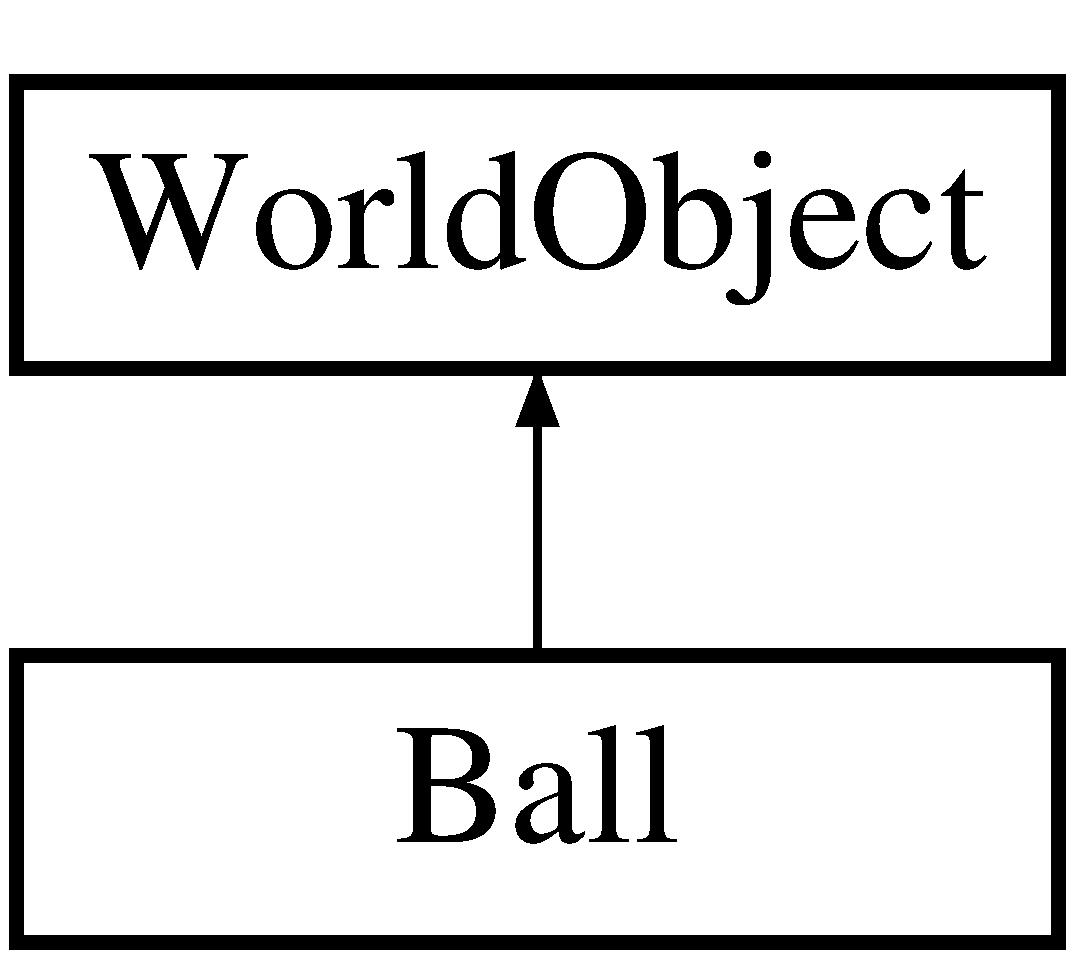
\includegraphics[height=2.000000cm]{class_ball}
\end{center}
\end{figure}
\subsection*{Public Member Functions}
\begin{DoxyCompactItemize}
\item 
\hypertarget{class_ball_a5b02c078ccc7dc50db406cc6afee22cd}{{\bfseries Ball} (\hyperlink{struct_point3_d}{Point3\+D} initial\+Direction, double speed, G\+Lfloat radius)}\label{class_ball_a5b02c078ccc7dc50db406cc6afee22cd}

\item 
\hypertarget{class_ball_a6bc4fe06d40ae8bb833cd758a6bca1ab}{void {\bfseries Draw\+Object} ()}\label{class_ball_a6bc4fe06d40ae8bb833cd758a6bca1ab}

\item 
\hypertarget{class_ball_ad4e6eac0cd9afd3d2be2267d6befe18a}{\hyperlink{struct_point3_d}{Point3\+D} {\bfseries Get\+Direction} ()}\label{class_ball_ad4e6eac0cd9afd3d2be2267d6befe18a}

\item 
\hypertarget{class_ball_ad56e662d67b4135c43cd637be246cf78}{void {\bfseries Move\+Left} (\hyperlink{struct_point3_d}{Point3\+D} on\+Track)}\label{class_ball_ad56e662d67b4135c43cd637be246cf78}

\item 
\hypertarget{class_ball_ace7571918ebb61526c6b30b7a2ecb711}{void {\bfseries Move\+Right} (\hyperlink{struct_point3_d}{Point3\+D} on\+Track)}\label{class_ball_ace7571918ebb61526c6b30b7a2ecb711}

\item 
\hypertarget{class_ball_a61798e313a118de5943221531255cf7a}{void {\bfseries Move\+Forward} ()}\label{class_ball_a61798e313a118de5943221531255cf7a}

\end{DoxyCompactItemize}
\subsection*{Additional Inherited Members}


The documentation for this class was generated from the following files\+:\begin{DoxyCompactItemize}
\item 
Ball.\+h\item 
Ball.\+cpp\end{DoxyCompactItemize}

\hypertarget{class_cactus}{\section{Cactus Class Reference}
\label{class_cactus}\index{Cactus@{Cactus}}
}


Derived from \hyperlink{class_plant}{Plant} class, indicates the pattern for creating each set of top points and the difference between each top's and base's radius.  




{\ttfamily \#include $<$Cactus.\+h$>$}

Inheritance diagram for Cactus\+:\begin{figure}[H]
\begin{center}
\leavevmode
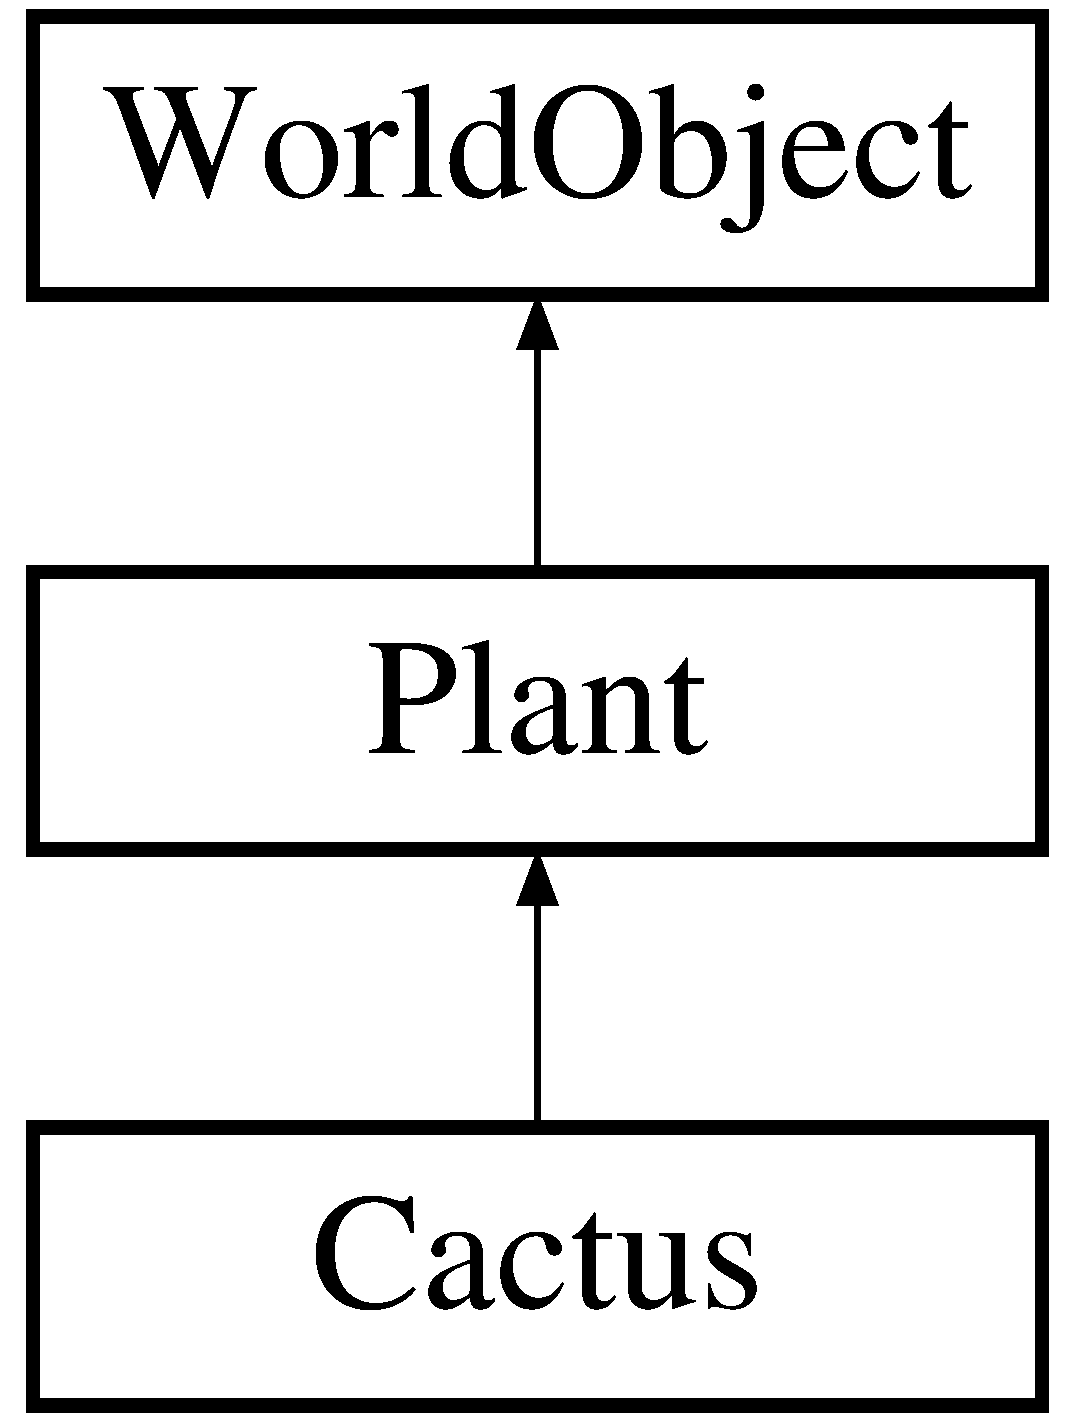
\includegraphics[height=3.000000cm]{class_cactus}
\end{center}
\end{figure}
\subsection*{Public Member Functions}
\begin{DoxyCompactItemize}
\item 
\hyperlink{class_cactus_a93bded0d899fc3b89e6be5f010d210e9}{Cactus} (double width, double height, int \hyperlink{class_plant_a4f86c46865d6211636140cef8805c6ee}{number\+Of\+Branches}, int \hyperlink{class_plant_ab49e92a2ab4ecdc762b5a1711fa3d65f}{level})
\item 
void \hyperlink{class_cactus_ae39a9e242e327a3f6c89126fb6d24a6b}{Set\+Branch\+Top} (vector$<$ \hyperlink{struct_point3_d}{Point3\+D} $>$ base, vector$<$ \hyperlink{struct_point3_d}{Point3\+D} $>$ \&top, int current\+Level, G\+Lfloat \hyperlink{class_plant_abef0f751fe6b1b43ed208966a70b4ab3}{radius}, G\+Lfloat pass, G\+Lfloat index)
\item 
void \hyperlink{class_cactus_a4a302b89f9c3ff94ac749bc870728c9e}{Set\+Initial\+Pass} (G\+Lfloat \&pass, G\+Lfloat \hyperlink{class_plant_abef0f751fe6b1b43ed208966a70b4ab3}{radius})
\item 
void \hyperlink{class_cactus_ae13abc19633a73f5647fb7da08b87faa}{Increment\+Pass} (G\+Lfloat \&pass, G\+Lfloat \hyperlink{class_plant_abef0f751fe6b1b43ed208966a70b4ab3}{radius})
\end{DoxyCompactItemize}
\subsection*{Additional Inherited Members}


\subsection{Detailed Description}
Derived from \hyperlink{class_plant}{Plant} class, indicates the pattern for creating each set of top points and the difference between each top's and base's radius. 

\subsection{Constructor \& Destructor Documentation}
\hypertarget{class_cactus_a93bded0d899fc3b89e6be5f010d210e9}{\index{Cactus@{Cactus}!Cactus@{Cactus}}
\index{Cactus@{Cactus}!Cactus@{Cactus}}
\subsubsection[{Cactus}]{\setlength{\rightskip}{0pt plus 5cm}Cactus\+::\+Cactus (
\begin{DoxyParamCaption}
\item[{double}]{width, }
\item[{double}]{height, }
\item[{int}]{number\+Of\+Branches, }
\item[{int}]{level}
\end{DoxyParamCaption}
)}}\label{class_cactus_a93bded0d899fc3b89e6be5f010d210e9}
\hyperlink{class_cactus}{Cactus}'s constructor 
\begin{DoxyParams}{Parameters}
{\em width} & double -- The width of the surface \\
\hline
{\em height} & double -- The height of the surface \\
\hline
{\em number\+Of\+Branches} & int -- The number of branches \\
\hline
{\em level} & int -- The levels of branches \\
\hline
\end{DoxyParams}
Initializes the texture index. Generates a random value for the maximum height. Generates random values for directions, each branch's radius and angles for the rotations around Y and Z axis. Calculate the maximum height for the current branch. Generates the maximum heights for each branch.

\subsection{Member Function Documentation}
\hypertarget{class_cactus_ae13abc19633a73f5647fb7da08b87faa}{\index{Cactus@{Cactus}!Increment\+Pass@{Increment\+Pass}}
\index{Increment\+Pass@{Increment\+Pass}!Cactus@{Cactus}}
\subsubsection[{Increment\+Pass}]{\setlength{\rightskip}{0pt plus 5cm}void Cactus\+::\+Increment\+Pass (
\begin{DoxyParamCaption}
\item[{G\+Lfloat \&}]{pass, }
\item[{G\+Lfloat}]{radius}
\end{DoxyParamCaption}
)\hspace{0.3cm}{\ttfamily [virtual]}}}\label{class_cactus_ae13abc19633a73f5647fb7da08b87faa}
Sets the value for incrementing the pass. 

Implements \hyperlink{class_plant}{Plant}.

\hypertarget{class_cactus_ae39a9e242e327a3f6c89126fb6d24a6b}{\index{Cactus@{Cactus}!Set\+Branch\+Top@{Set\+Branch\+Top}}
\index{Set\+Branch\+Top@{Set\+Branch\+Top}!Cactus@{Cactus}}
\subsubsection[{Set\+Branch\+Top}]{\setlength{\rightskip}{0pt plus 5cm}void Cactus\+::\+Set\+Branch\+Top (
\begin{DoxyParamCaption}
\item[{vector$<$ {\bf Point3\+D} $>$}]{base, }
\item[{vector$<$ {\bf Point3\+D} $>$ \&}]{top, }
\item[{int}]{current\+Level, }
\item[{G\+Lfloat}]{radius, }
\item[{G\+Lfloat}]{pass, }
\item[{G\+Lfloat}]{index}
\end{DoxyParamCaption}
)\hspace{0.3cm}{\ttfamily [virtual]}}}\label{class_cactus_ae39a9e242e327a3f6c89126fb6d24a6b}
Initializes a vector of top points using a given base, its radius and a pass. 
\begin{DoxyParams}{Parameters}
{\em base} & vector$<$\+Point3\+D$>$ -- A vector that stores the points of the base of the branch \\
\hline
{\em top} & vector$<$\+Point3\+D$>$ -- A vector that will be initialized with the points of the top of the branch \\
\hline
{\em current\+Level} & int -- The current level of branches \\
\hline
{\em radius} & G\+Lfloat -- The radius of the base \\
\hline
{\em pass} & G\+Lfloat -- The difference between the radius of the base and the radius of the top \\
\hline
{\em index} & G\+Lfloat -- The index of the branch \\
\hline
\end{DoxyParams}
Calculates the difference between each top and base.

Sets the difference on the X axis for the first half of branches.

Increments the current radius so that each top's radius will be bigger than the previous one.

Initializes the top points on the left/right side according to the corresponding direction(1-\/left, 2-\/right).

If the current branch is the stem(current\+Level=1), the radius of the top will not be bigger than the base.\+Otherwise, the radius of the top will be bigger than the base.

Implements \hyperlink{class_plant}{Plant}.

\hypertarget{class_cactus_a4a302b89f9c3ff94ac749bc870728c9e}{\index{Cactus@{Cactus}!Set\+Initial\+Pass@{Set\+Initial\+Pass}}
\index{Set\+Initial\+Pass@{Set\+Initial\+Pass}!Cactus@{Cactus}}
\subsubsection[{Set\+Initial\+Pass}]{\setlength{\rightskip}{0pt plus 5cm}void Cactus\+::\+Set\+Initial\+Pass (
\begin{DoxyParamCaption}
\item[{G\+Lfloat \&}]{pass, }
\item[{G\+Lfloat}]{radius}
\end{DoxyParamCaption}
)\hspace{0.3cm}{\ttfamily [virtual]}}}\label{class_cactus_a4a302b89f9c3ff94ac749bc870728c9e}
Initializes the difference between top's and base's radius. 
\begin{DoxyParams}{Parameters}
{\em radius} & G\+Lfloat -- The radius of the base \\
\hline
{\em pass} & G\+Lfloat -- The difference between the radius of the base and the radius of the top \\
\hline
\end{DoxyParams}


Implements \hyperlink{class_plant}{Plant}.



The documentation for this class was generated from the following files\+:\begin{DoxyCompactItemize}
\item 
Cactus.\+h\item 
Cactus.\+cpp\end{DoxyCompactItemize}

\hypertarget{class_camera}{\section{Camera Class Reference}
\label{class_camera}\index{Camera@{Camera}}
}
Inheritance diagram for Camera\+:\begin{figure}[H]
\begin{center}
\leavevmode
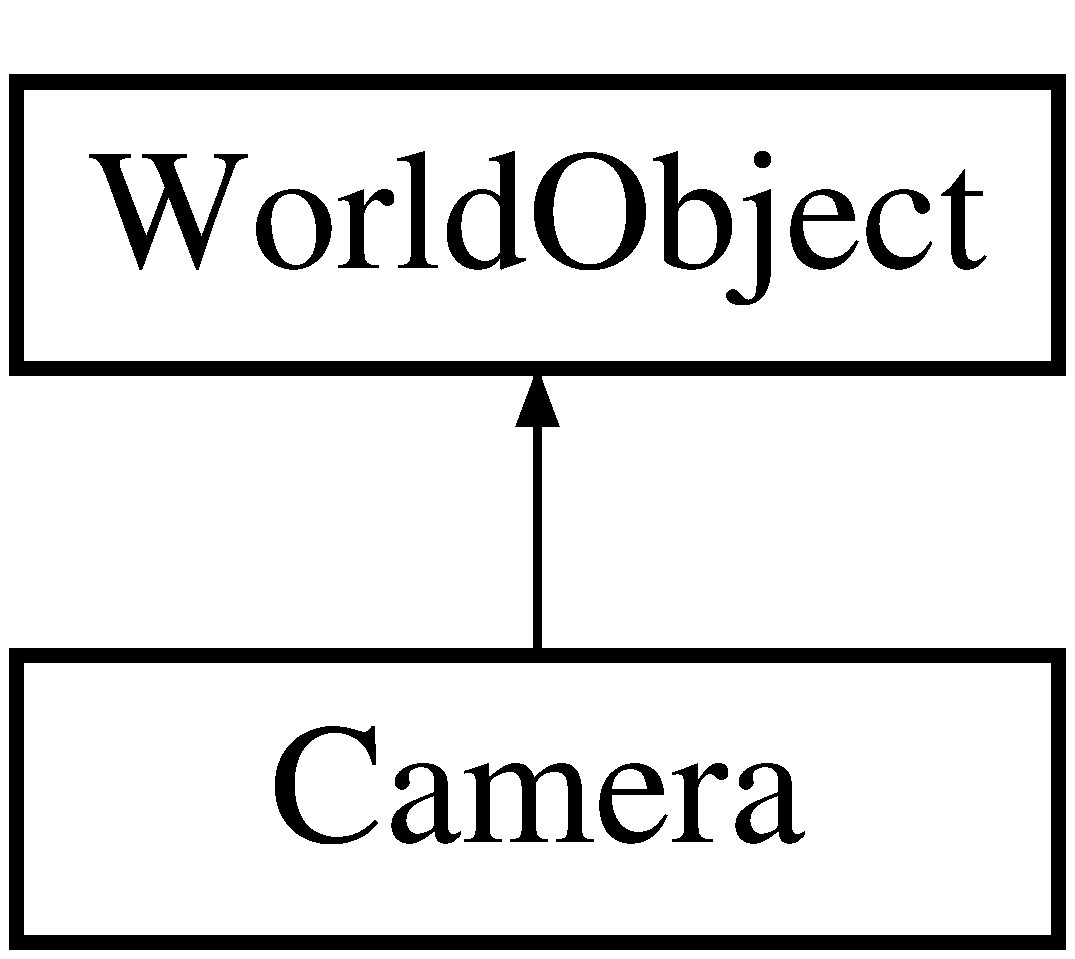
\includegraphics[height=2.000000cm]{class_camera}
\end{center}
\end{figure}
\subsection*{Public Member Functions}
\begin{DoxyCompactItemize}
\item 
\hypertarget{class_camera_aa2f1b00493b49201482e3836d8969d08}{void {\bfseries Perspective} ()}\label{class_camera_aa2f1b00493b49201482e3836d8969d08}

\item 
\hypertarget{class_camera_a8a49e140cb548b3fc11c61c8f48214c4}{void {\bfseries Follow} (\hyperlink{class_ball}{Ball} $\ast$ball)}\label{class_camera_a8a49e140cb548b3fc11c61c8f48214c4}

\item 
\hypertarget{class_camera_a8161f7e096c69039c67d55661abb85f6}{void {\bfseries Un\+Follow} ()}\label{class_camera_a8161f7e096c69039c67d55661abb85f6}

\item 
\hypertarget{class_camera_a4a596a3ea1fdc7d244ba4268031a360b}{void {\bfseries Update} ()}\label{class_camera_a4a596a3ea1fdc7d244ba4268031a360b}

\end{DoxyCompactItemize}
\subsection*{Protected Member Functions}
\begin{DoxyCompactItemize}
\item 
\hypertarget{class_camera_ac8552e15d6c3eabd50ddf300520ca8a1}{void {\bfseries Draw\+Object} ()}\label{class_camera_ac8552e15d6c3eabd50ddf300520ca8a1}

\end{DoxyCompactItemize}
\subsection*{Protected Attributes}
\begin{DoxyCompactItemize}
\item 
\hypertarget{class_camera_a6969c8a06de8be781e79039c560895aa}{\hyperlink{struct_point3_d}{Point3\+D} {\bfseries direction}}\label{class_camera_a6969c8a06de8be781e79039c560895aa}

\item 
\hypertarget{class_camera_ac949c9480f9e1935fcfe31b1b88f12bb}{\hyperlink{class_ball}{Ball} $\ast$ {\bfseries ball}}\label{class_camera_ac949c9480f9e1935fcfe31b1b88f12bb}

\end{DoxyCompactItemize}


The documentation for this class was generated from the following files\+:\begin{DoxyCompactItemize}
\item 
Camera.\+h\item 
Camera.\+cpp\end{DoxyCompactItemize}

\hypertarget{class_corner}{\section{Corner Class Reference}
\label{class_corner}\index{Corner@{Corner}}
}
\subsection*{Public Member Functions}
\begin{DoxyCompactItemize}
\item 
\hypertarget{class_corner_ab55d2cbce25b09663c8df9bb9ac2210f}{{\bfseries Corner} (\hyperlink{struct_point3_d}{Point3\+D} point, bool left, bool right, G\+Lfloat radius=8.\+0)}\label{class_corner_ab55d2cbce25b09663c8df9bb9ac2210f}

\item 
\hypertarget{class_corner_a4148b59b83d2b9cad19ec13f234766a8}{bool {\bfseries Can\+Move\+Left} (\hyperlink{class_ball}{Ball} $\ast$ball)}\label{class_corner_a4148b59b83d2b9cad19ec13f234766a8}

\item 
\hypertarget{class_corner_a533010b03b15b6c76ad0a9f534018a8c}{bool {\bfseries Can\+Move\+Right} (\hyperlink{class_ball}{Ball} $\ast$ball)}\label{class_corner_a533010b03b15b6c76ad0a9f534018a8c}

\item 
\hypertarget{class_corner_a615f08b3eb5490bdfedf5ca0c1a8f730}{\hyperlink{struct_point3_d}{Point3\+D} {\bfseries Get\+Point} ()}\label{class_corner_a615f08b3eb5490bdfedf5ca0c1a8f730}

\item 
\hypertarget{class_corner_a6fa76d41c90f1684f53e8ceee402ccdb}{G\+Lfloat {\bfseries Get\+Radius} ()}\label{class_corner_a6fa76d41c90f1684f53e8ceee402ccdb}

\end{DoxyCompactItemize}


The documentation for this class was generated from the following files\+:\begin{DoxyCompactItemize}
\item 
Corner.\+h\item 
Corner.\+cpp\end{DoxyCompactItemize}

\hypertarget{class_curve}{\section{Curve Class Reference}
\label{class_curve}\index{Curve@{Curve}}
}
Inheritance diagram for Curve\+:\begin{figure}[H]
\begin{center}
\leavevmode
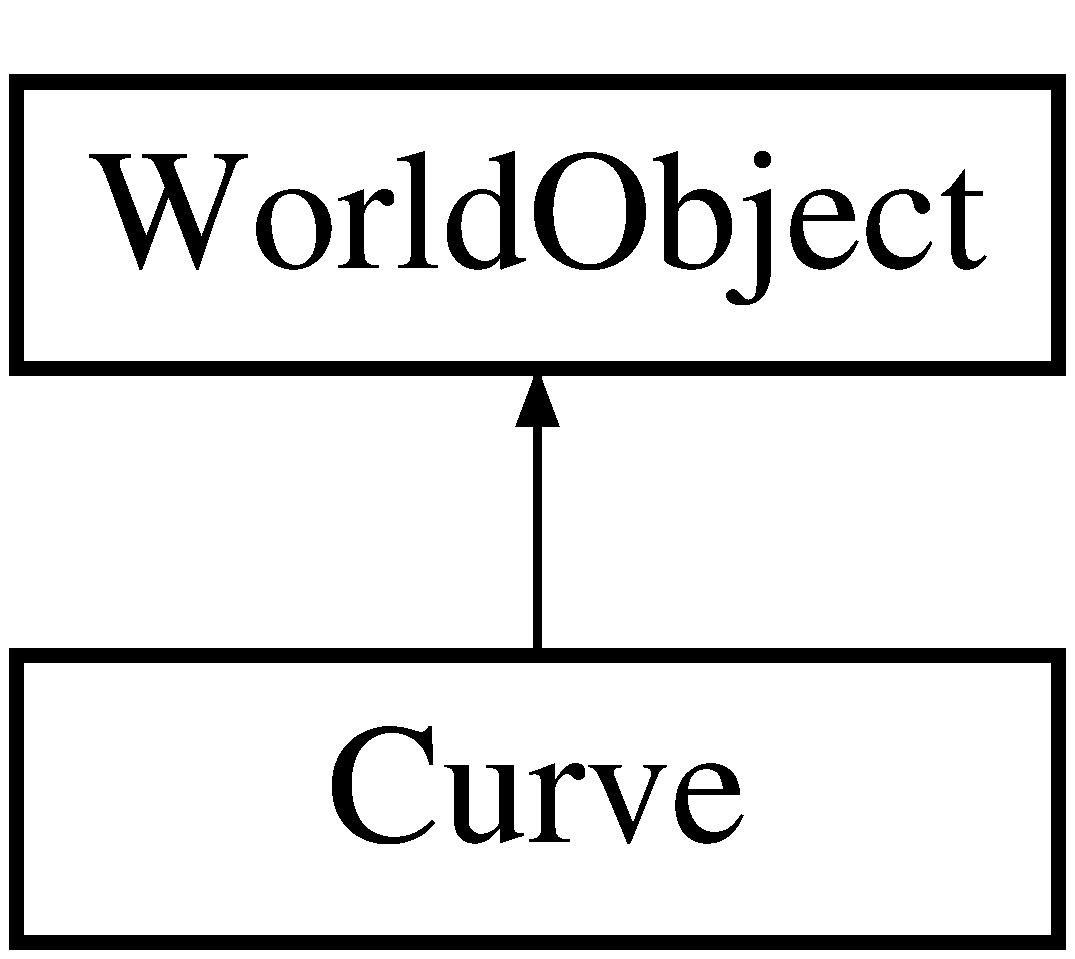
\includegraphics[height=2.000000cm]{class_curve}
\end{center}
\end{figure}
\subsection*{Public Member Functions}
\begin{DoxyCompactItemize}
\item 
\hypertarget{class_curve_a25ea22fdfb1642309a758bf05829b77e}{{\bfseries Curve} (int T\+U\+R\+N)}\label{class_curve_a25ea22fdfb1642309a758bf05829b77e}

\end{DoxyCompactItemize}
\subsection*{Additional Inherited Members}


The documentation for this class was generated from the following files\+:\begin{DoxyCompactItemize}
\item 
Curve.\+h\item 
Curve.\+cpp\end{DoxyCompactItemize}

\hypertarget{class_digit}{\section{Digit Class Reference}
\label{class_digit}\index{Digit@{Digit}}
}
Inheritance diagram for Digit\+:\begin{figure}[H]
\begin{center}
\leavevmode
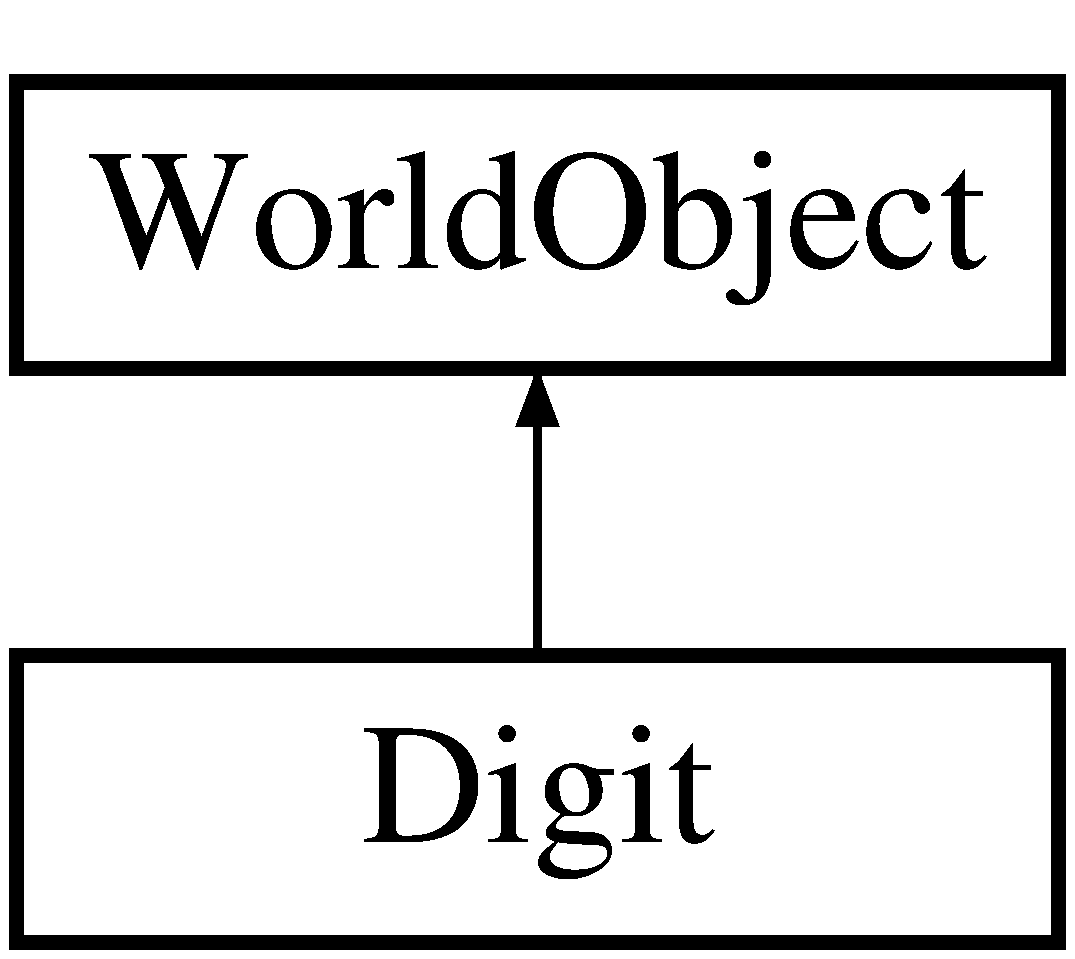
\includegraphics[height=2.000000cm]{class_digit}
\end{center}
\end{figure}
\subsection*{Public Member Functions}
\begin{DoxyCompactItemize}
\item 
\hypertarget{class_digit_ac26a02f08c1ea432947616ffd27e9858}{{\bfseries Digit} (int digit)}\label{class_digit_ac26a02f08c1ea432947616ffd27e9858}

\item 
\hypertarget{class_digit_ae67a2c0b0a951a31b8a618911b87f0bc}{void {\bfseries Follow} (\hyperlink{class_ball}{Ball} $\ast$ball, \hyperlink{struct_point3_d}{Point3\+D} follow\+Point)}\label{class_digit_ae67a2c0b0a951a31b8a618911b87f0bc}

\item 
\hypertarget{class_digit_a00d932e15f940d2e1e1da94bdeaa498a}{void {\bfseries Update} ()}\label{class_digit_a00d932e15f940d2e1e1da94bdeaa498a}

\item 
\hypertarget{class_digit_a528791513a2feaa3e96b12475f86843f}{void {\bfseries Set\+Digit} (double digit)}\label{class_digit_a528791513a2feaa3e96b12475f86843f}

\end{DoxyCompactItemize}
\subsection*{Additional Inherited Members}


The documentation for this class was generated from the following files\+:\begin{DoxyCompactItemize}
\item 
Digit.\+h\item 
Digit.\+cpp\end{DoxyCompactItemize}

\hypertarget{class_earth}{\section{Earth Class Reference}
\label{class_earth}\index{Earth@{Earth}}
}
Inheritance diagram for Earth\+:\begin{figure}[H]
\begin{center}
\leavevmode
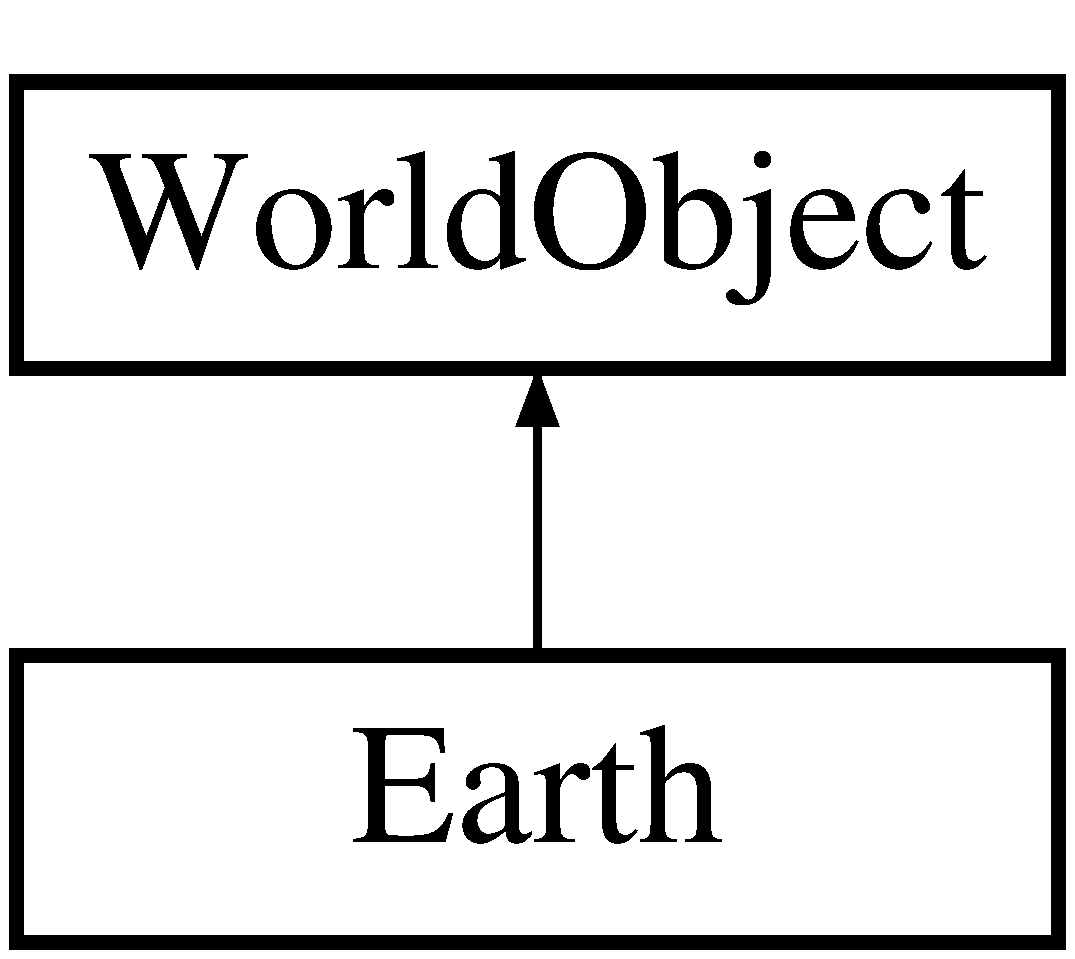
\includegraphics[height=2.000000cm]{class_earth}
\end{center}
\end{figure}
\subsection*{Public Member Functions}
\begin{DoxyCompactItemize}
\item 
\hypertarget{class_earth_a3e7410e27847c21aa17b4322103d1e00}{void {\bfseries Draw\+Object} ()}\label{class_earth_a3e7410e27847c21aa17b4322103d1e00}

\end{DoxyCompactItemize}
\subsection*{Additional Inherited Members}


The documentation for this class was generated from the following files\+:\begin{DoxyCompactItemize}
\item 
Earth.\+h\item 
Earth.\+cpp\end{DoxyCompactItemize}

\hypertarget{class_end_screen}{\section{End\+Screen Class Reference}
\label{class_end_screen}\index{End\+Screen@{End\+Screen}}
}
Inheritance diagram for End\+Screen\+:\begin{figure}[H]
\begin{center}
\leavevmode
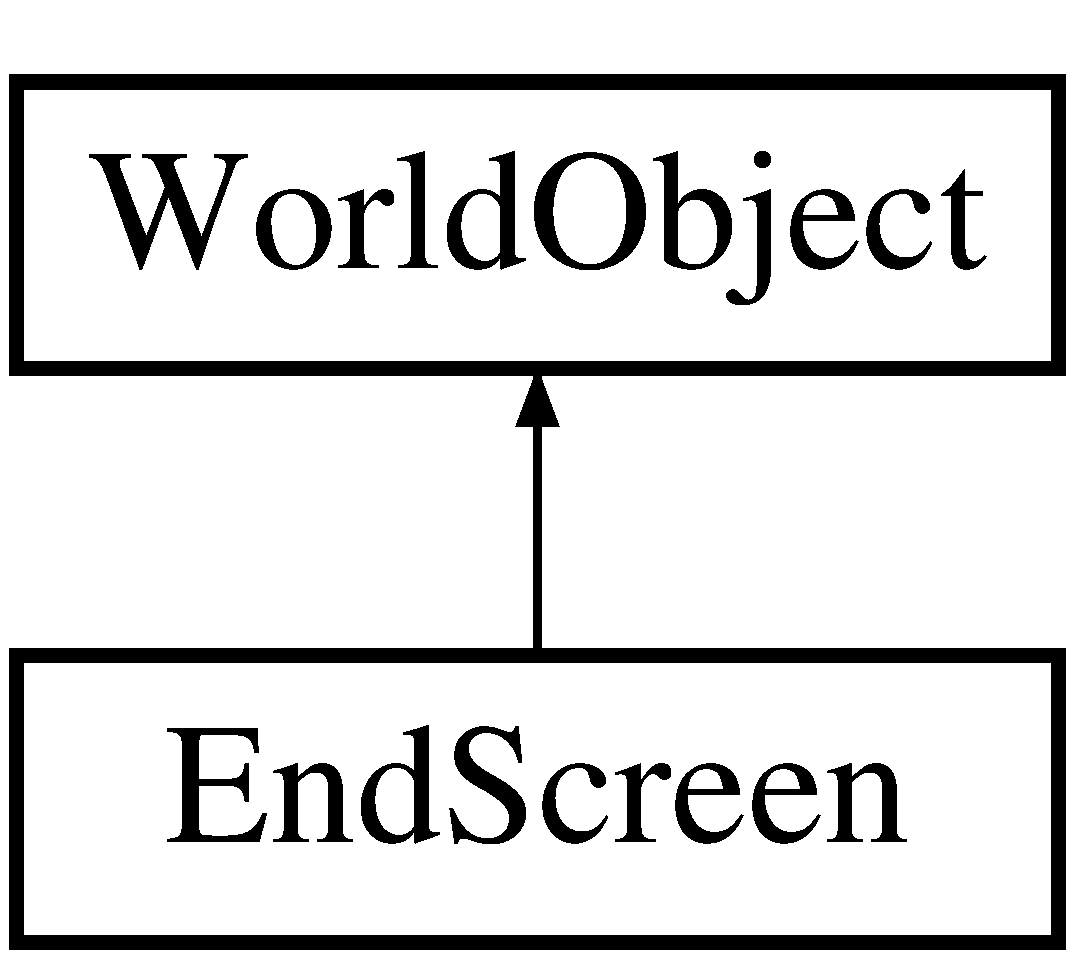
\includegraphics[height=2.000000cm]{class_end_screen}
\end{center}
\end{figure}
\subsection*{Additional Inherited Members}


The documentation for this class was generated from the following files\+:\begin{DoxyCompactItemize}
\item 
End\+Screen.\+h\item 
End\+Screen.\+cpp\end{DoxyCompactItemize}

\hypertarget{class_highway}{\section{Highway Class Reference}
\label{class_highway}\index{Highway@{Highway}}
}
Inheritance diagram for Highway\+:\begin{figure}[H]
\begin{center}
\leavevmode
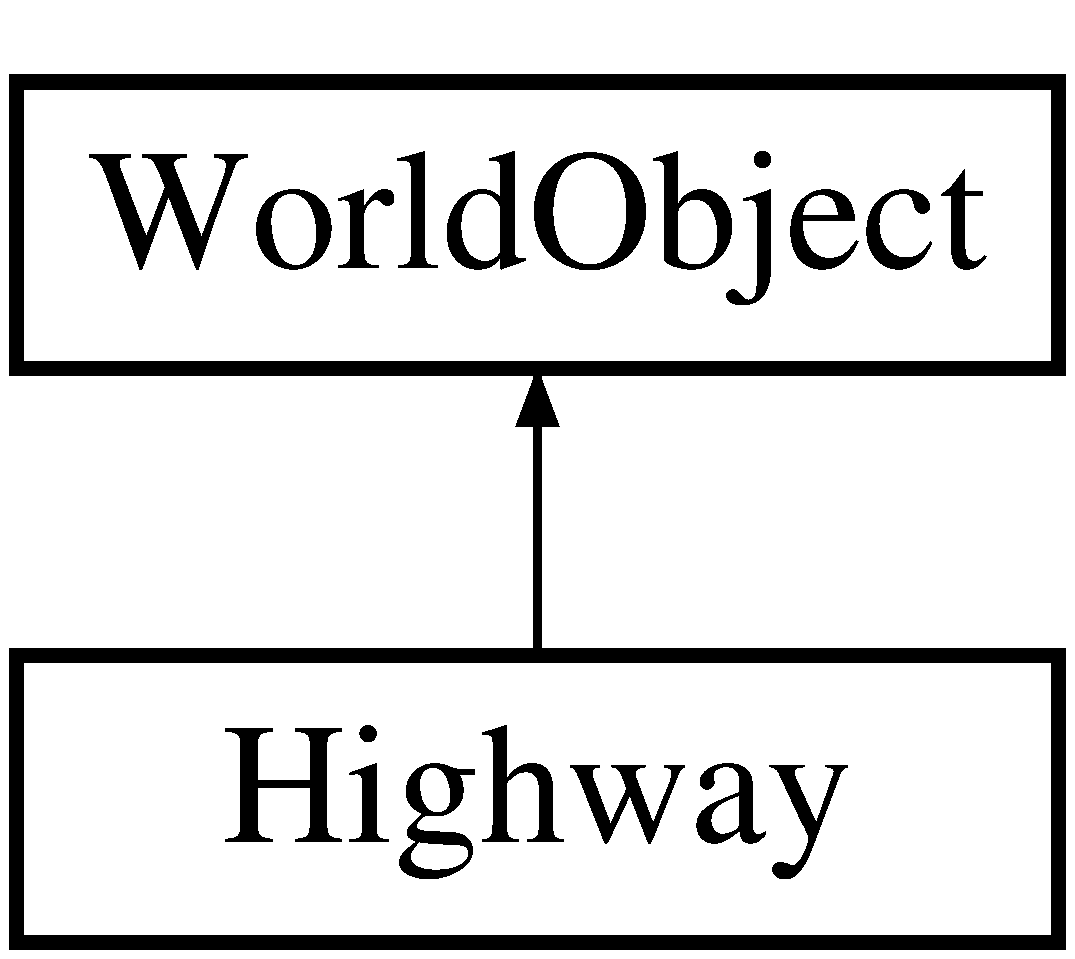
\includegraphics[height=2.000000cm]{class_highway}
\end{center}
\end{figure}
\subsection*{Public Member Functions}
\begin{DoxyCompactItemize}
\item 
\hypertarget{class_highway_abcdc42e3d3d0131e20857de0428ebe57}{{\bfseries Highway} (\hyperlink{class_scene}{Scene} $\ast$scene)}\label{class_highway_abcdc42e3d3d0131e20857de0428ebe57}

\item 
\hypertarget{class_highway_a04fe3235ee2707ad5c9043c38983a720}{void {\bfseries Follow} (\hyperlink{class_ball}{Ball} $\ast$ball)}\label{class_highway_a04fe3235ee2707ad5c9043c38983a720}

\item 
\hypertarget{class_highway_a71284d072685662c59591f804248dc89}{void {\bfseries Update} ()}\label{class_highway_a71284d072685662c59591f804248dc89}

\item 
\hypertarget{class_highway_a1a6e351d6c701e823052f69d233fb4de}{bool {\bfseries Can\+Move\+Left} (\hyperlink{struct_point3_d}{Point3\+D} \&point)}\label{class_highway_a1a6e351d6c701e823052f69d233fb4de}

\item 
\hypertarget{class_highway_a94e2179430243fef55e8459f891326ac}{bool {\bfseries Can\+Move\+Right} (\hyperlink{struct_point3_d}{Point3\+D} \&point)}\label{class_highway_a94e2179430243fef55e8459f891326ac}

\item 
\hypertarget{class_highway_a826881d3a7e1332f7d16deb5b7f998dd}{bool {\bfseries Is\+Off\+Road} ()}\label{class_highway_a826881d3a7e1332f7d16deb5b7f998dd}

\end{DoxyCompactItemize}
\subsection*{Additional Inherited Members}


The documentation for this class was generated from the following files\+:\begin{DoxyCompactItemize}
\item 
Highway.\+h\item 
Highway.\+cpp\end{DoxyCompactItemize}

\hypertarget{class_mountain}{\section{Mountain Class Reference}
\label{class_mountain}\index{Mountain@{Mountain}}
}
Inheritance diagram for Mountain\+:\begin{figure}[H]
\begin{center}
\leavevmode
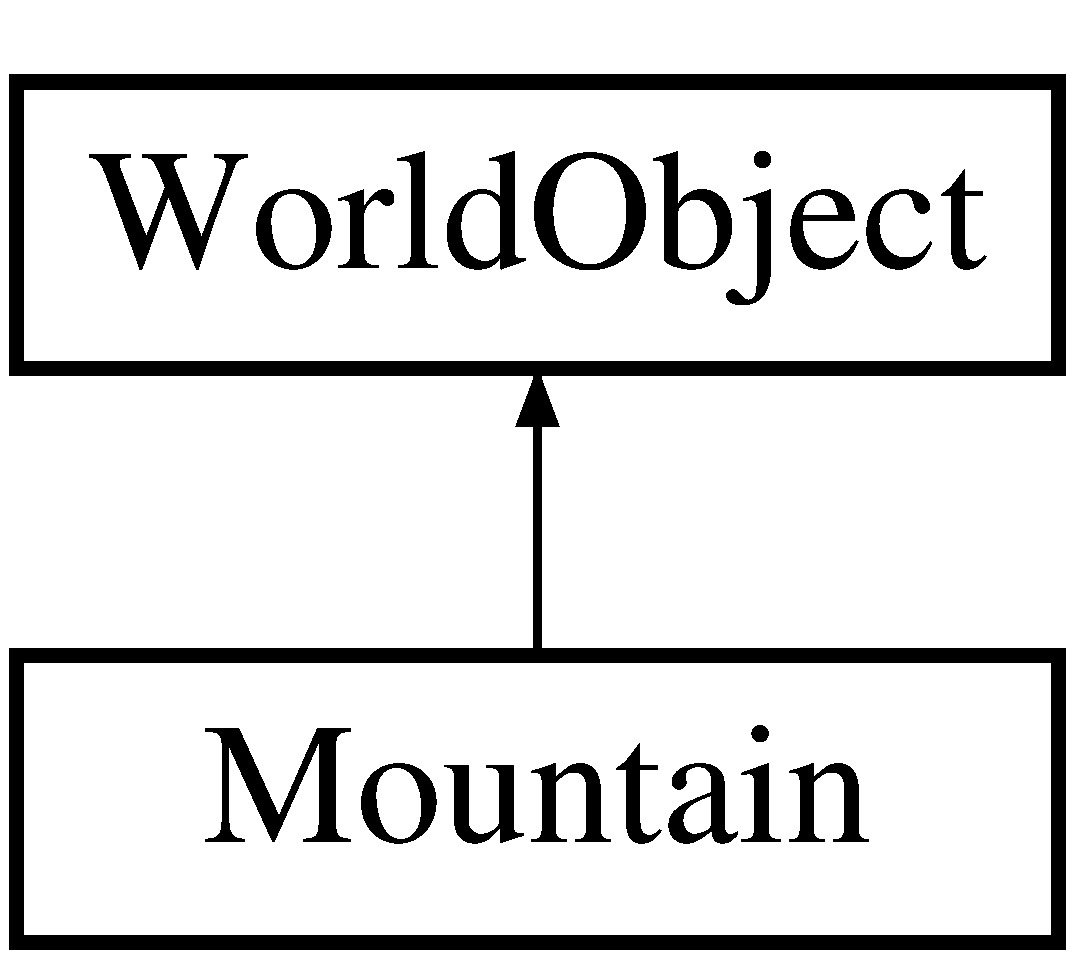
\includegraphics[height=2.000000cm]{class_mountain}
\end{center}
\end{figure}
\subsection*{Public Member Functions}
\begin{DoxyCompactItemize}
\item 
\hypertarget{class_mountain_a32ddb9ae59bd166cf3059fddef8061cd}{{\bfseries Mountain} (G\+Lfloat width, G\+Lfloat height, G\+Lfloat inaltime)}\label{class_mountain_a32ddb9ae59bd166cf3059fddef8061cd}

\item 
\hypertarget{class_mountain_a146cf4314092e1c6cbfa957724476af0}{void {\bfseries Draw\+Object} ()}\label{class_mountain_a146cf4314092e1c6cbfa957724476af0}

\end{DoxyCompactItemize}
\subsection*{Additional Inherited Members}


The documentation for this class was generated from the following files\+:\begin{DoxyCompactItemize}
\item 
Mountain.\+h\item 
Mountain.\+cpp\end{DoxyCompactItemize}

\hypertarget{class_plant}{\section{Plant Class Reference}
\label{class_plant}\index{Plant@{Plant}}
}


Abstract class, indicates the way a branch will be drawn.  




{\ttfamily \#include $<$Plant.\+h$>$}

Inheritance diagram for Plant\+:\begin{figure}[H]
\begin{center}
\leavevmode
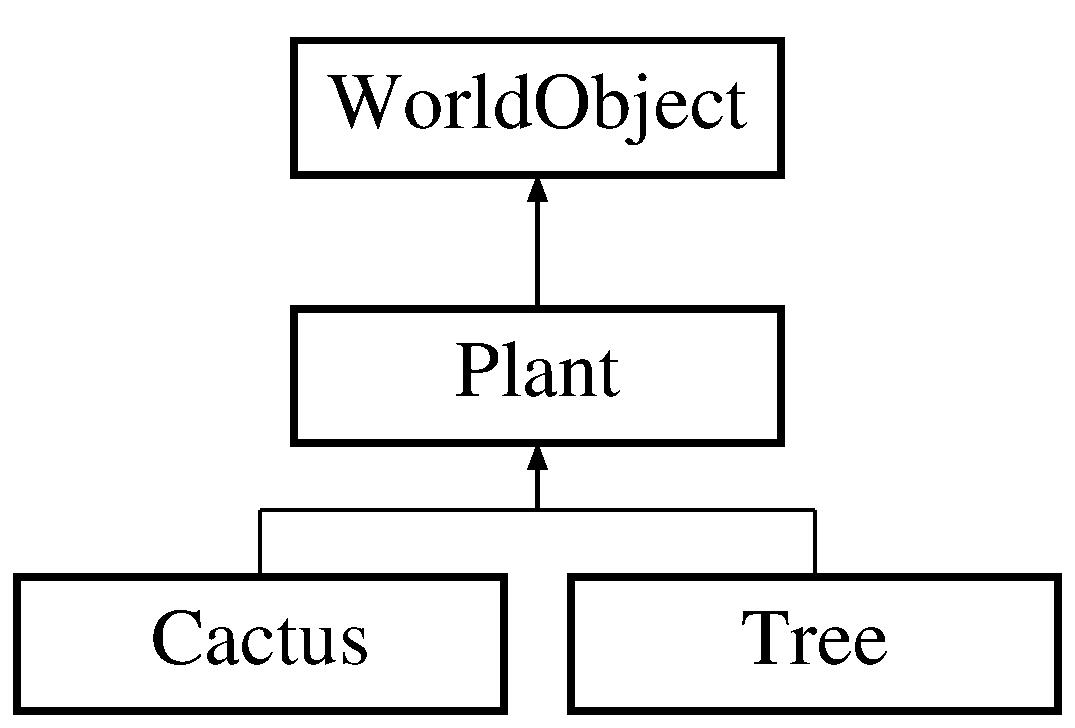
\includegraphics[height=3.000000cm]{class_plant}
\end{center}
\end{figure}
\subsection*{Public Member Functions}
\begin{DoxyCompactItemize}
\item 
\hyperlink{class_plant_ac5fefc6f365188701cbc72d92ca42af1}{Plant} (double width, double height, int \hyperlink{class_plant_a4f86c46865d6211636140cef8805c6ee}{number\+Of\+Branches}, int \hyperlink{class_plant_ab49e92a2ab4ecdc762b5a1711fa3d65f}{level})
\item 
\hyperlink{class_plant_ac63f88c71ee3a3da6d6bdcf0111268e1}{$\sim$\+Plant} (void)
\item 
void \hyperlink{class_plant_ac04e2a45a28c7fa0d97b3c764128c9e5}{Draw\+Object} ()
\item 
void \hyperlink{class_plant_ac4b9655b2932b5dab8cc67671ca9e89f}{Draw\+Branch} (vector$<$ \hyperlink{struct_point3_d}{Point3\+D} $>$base, G\+Lfloat \hyperlink{class_plant_abef0f751fe6b1b43ed208966a70b4ab3}{radius}, int current\+Level)
\item 
void \hyperlink{class_plant_a8d678cebc0b25205820d111a27d90344}{Put\+Texture\+On\+Cylinder} (vector$<$ \hyperlink{struct_point3_d}{Point3\+D} $>$ base, vector$<$ \hyperlink{struct_point3_d}{Point3\+D} $>$ top)
\item 
\hypertarget{class_plant_a9660240dc434e603ea26335eed9e3c7a}{virtual void {\bfseries Set\+Branch\+Top} (vector$<$ \hyperlink{struct_point3_d}{Point3\+D} $>$ base, vector$<$ \hyperlink{struct_point3_d}{Point3\+D} $>$ \&top, int current\+Level, G\+Lfloat \hyperlink{class_plant_abef0f751fe6b1b43ed208966a70b4ab3}{radius}, G\+Lfloat pass, G\+Lfloat index)=0}\label{class_plant_a9660240dc434e603ea26335eed9e3c7a}

\item 
\hypertarget{class_plant_a66954b597c49fc536cebe914697b762b}{virtual void {\bfseries Set\+Initial\+Pass} (G\+Lfloat \&pass, G\+Lfloat \hyperlink{class_plant_abef0f751fe6b1b43ed208966a70b4ab3}{radius})=0}\label{class_plant_a66954b597c49fc536cebe914697b762b}

\item 
\hypertarget{class_plant_a77a88d6d25e58b0cf9bd5f6aaa5d9572}{virtual void {\bfseries Increment\+Pass} (G\+Lfloat \&pass, G\+Lfloat \hyperlink{class_plant_abef0f751fe6b1b43ed208966a70b4ab3}{radius})=0}\label{class_plant_a77a88d6d25e58b0cf9bd5f6aaa5d9572}

\end{DoxyCompactItemize}
\subsection*{Protected Attributes}
\begin{DoxyCompactItemize}
\item 
G\+Lfloat \hyperlink{class_plant_abef0f751fe6b1b43ed208966a70b4ab3}{radius}
\item 
G\+Lfloat \hyperlink{class_plant_a71a5a857d8a0adcfb612dadfcfffc731}{max\+Height}
\item 
vector$<$ G\+Lfloat $>$ \hyperlink{class_plant_a16888c602067089a5aaa25ab6a92466f}{angles\+Y}
\item 
vector$<$ G\+Lfloat $>$ \hyperlink{class_plant_a298b462dbd0b350d08b5262990a2576b}{angles\+Z}
\item 
vector$<$ G\+Lfloat $>$ \hyperlink{class_plant_a4d8a4ea7bbede32b0f6ba1f3415d8f54}{branches\+Radius}
\item 
vector$<$ int $>$ \hyperlink{class_plant_a3ec2334fa4c49998f74f62240eaf7537}{directions}
\item 
vector$<$ G\+Lfloat $>$ \hyperlink{class_plant_aa12026d894eba8a2764d5edf94757850}{heights}
\item 
int \hyperlink{class_plant_a4f86c46865d6211636140cef8805c6ee}{number\+Of\+Branches}
\item 
int \hyperlink{class_plant_aeaaf035b21354b12a272f66db178f5cb}{texture\+Index}
\item 
int \hyperlink{class_plant_ab49e92a2ab4ecdc762b5a1711fa3d65f}{level}
\end{DoxyCompactItemize}
\subsection*{Friends}
\begin{DoxyCompactItemize}
\item 
G\+Lfloat \hyperlink{class_plant_a38de3a3700e430ebecffa518977d2880}{Get\+Random\+G\+Lfloat} (G\+Lfloat min, G\+Lfloat max)
\end{DoxyCompactItemize}
\subsection*{Additional Inherited Members}


\subsection{Detailed Description}
Abstract class, indicates the way a branch will be drawn. 

\subsection{Constructor \& Destructor Documentation}
\hypertarget{class_plant_ac5fefc6f365188701cbc72d92ca42af1}{\index{Plant@{Plant}!Plant@{Plant}}
\index{Plant@{Plant}!Plant@{Plant}}
\subsubsection[{Plant}]{\setlength{\rightskip}{0pt plus 5cm}Plant\+::\+Plant (
\begin{DoxyParamCaption}
\item[{double}]{width, }
\item[{double}]{height, }
\item[{int}]{number\+Of\+Branches, }
\item[{int}]{level}
\end{DoxyParamCaption}
)}}\label{class_plant_ac5fefc6f365188701cbc72d92ca42af1}
\hyperlink{class_plant}{Plant}'s constructor 
\begin{DoxyParams}{Parameters}
{\em width} & double -- The width of the surface \\
\hline
{\em height} & double -- The height of the surface \\
\hline
{\em number\+Of\+Branches} & int -- The number of branches \\
\hline
{\em level} & int -- The levels of branches \\
\hline
\end{DoxyParams}
Calculate the minimum between height and width. Generates a random value in \mbox{[}min\+Dimension/8, min\+Dimension/4\mbox{]} for the radius.\hypertarget{class_plant_ac63f88c71ee3a3da6d6bdcf0111268e1}{\index{Plant@{Plant}!````~Plant@{$\sim$\+Plant}}
\index{````~Plant@{$\sim$\+Plant}!Plant@{Plant}}
\subsubsection[{$\sim$\+Plant}]{\setlength{\rightskip}{0pt plus 5cm}Plant\+::$\sim$\+Plant (
\begin{DoxyParamCaption}
\item[{void}]{}
\end{DoxyParamCaption}
)}}\label{class_plant_ac63f88c71ee3a3da6d6bdcf0111268e1}
\hyperlink{class_plant}{Plant}'s destructor 

\subsection{Member Function Documentation}
\hypertarget{class_plant_ac4b9655b2932b5dab8cc67671ca9e89f}{\index{Plant@{Plant}!Draw\+Branch@{Draw\+Branch}}
\index{Draw\+Branch@{Draw\+Branch}!Plant@{Plant}}
\subsubsection[{Draw\+Branch}]{\setlength{\rightskip}{0pt plus 5cm}void Plant\+::\+Draw\+Branch (
\begin{DoxyParamCaption}
\item[{vector$<$ {\bf Point3\+D} $>$}]{base, }
\item[{G\+Lfloat}]{radius, }
\item[{int}]{current\+Level}
\end{DoxyParamCaption}
)}}\label{class_plant_ac4b9655b2932b5dab8cc67671ca9e89f}
Draw\+Branch method 
\begin{DoxyParams}{Parameters}
{\em base} & vector$<$\+Point3\+D$>$ -- A vector that stores the points of the base of the branch \\
\hline
{\em radius} & G\+Lfloat -- Base's radius of the branch \\
\hline
{\em current\+Level} & int -- The current level of branches \\
\hline
\end{DoxyParams}
Checks if the current level is the last one.

Draws the branch on the right side.

Make rotations around the Y and Z axis with the corresponding angles for the current branch if the current branch is not the last one.

Draws a branch of the current branch.

Make rotations around the Y and Z axis with the inverse angles of the previous rotation.

Draws the branch on the left side.

Make rotations around the Y and Z axis with the opposite angles corresponding to the left branch.

Draws a branch of the current branch.

Make rotations around the Y and Z axis with the opposite angles corresponding to the left branch.

The base will be replaced by the top, the top will be generated after.\hypertarget{class_plant_ac04e2a45a28c7fa0d97b3c764128c9e5}{\index{Plant@{Plant}!Draw\+Object@{Draw\+Object}}
\index{Draw\+Object@{Draw\+Object}!Plant@{Plant}}
\subsubsection[{Draw\+Object}]{\setlength{\rightskip}{0pt plus 5cm}void Plant\+::\+Draw\+Object (
\begin{DoxyParamCaption}
{}
\end{DoxyParamCaption}
)\hspace{0.3cm}{\ttfamily [virtual]}}}\label{class_plant_ac04e2a45a28c7fa0d97b3c764128c9e5}
Draw\+Object method Draws all branches of the plant. Generates the points of the initial base using the equation of an ellipse.

Implements \hyperlink{class_world_object}{World\+Object}.

\hypertarget{class_plant_a8d678cebc0b25205820d111a27d90344}{\index{Plant@{Plant}!Put\+Texture\+On\+Cylinder@{Put\+Texture\+On\+Cylinder}}
\index{Put\+Texture\+On\+Cylinder@{Put\+Texture\+On\+Cylinder}!Plant@{Plant}}
\subsubsection[{Put\+Texture\+On\+Cylinder}]{\setlength{\rightskip}{0pt plus 5cm}void Plant\+::\+Put\+Texture\+On\+Cylinder (
\begin{DoxyParamCaption}
\item[{vector$<$ {\bf Point3\+D} $>$}]{base, }
\item[{vector$<$ {\bf Point3\+D} $>$}]{top}
\end{DoxyParamCaption}
)}}\label{class_plant_a8d678cebc0b25205820d111a27d90344}
Put\+Texture\+On\+Cylinder Method Puts a texture on a cylinder based on its base points and its top points 
\begin{DoxyParams}{Parameters}
{\em base} & vector$<$\+Point3\+D$>$ -- A vector that stores the points of the base of the cylinder \\
\hline
{\em top} & vector$<$\+Point3\+D$>$ -- A vector that stores the points of the top of the cylinder \\
\hline
\end{DoxyParams}
Calculate the distance between two pixels of the texture.

Puts texture on each triangle based on each 2 points of the top and 1 point of the base.

Puts texture on the next triangle based on each 2 points of the base and 1 point of the top.

\subsection{Friends And Related Function Documentation}
\hypertarget{class_plant_a38de3a3700e430ebecffa518977d2880}{\index{Plant@{Plant}!Get\+Random\+G\+Lfloat@{Get\+Random\+G\+Lfloat}}
\index{Get\+Random\+G\+Lfloat@{Get\+Random\+G\+Lfloat}!Plant@{Plant}}
\subsubsection[{Get\+Random\+G\+Lfloat}]{\setlength{\rightskip}{0pt plus 5cm}G\+Lfloat Get\+Random\+G\+Lfloat (
\begin{DoxyParamCaption}
\item[{G\+Lfloat}]{min, }
\item[{G\+Lfloat}]{max}
\end{DoxyParamCaption}
)\hspace{0.3cm}{\ttfamily [friend]}}}\label{class_plant_a38de3a3700e430ebecffa518977d2880}
Draw\+Branch method 
\begin{DoxyParams}{Parameters}
{\em min} & G\+Lfloat -- The minimum value \\
\hline
{\em max} & G\+Lfloat -- The maximum value Generates a random value in \mbox{[}min, max\mbox{]}. \\
\hline
\end{DoxyParams}


\subsection{Member Data Documentation}
\hypertarget{class_plant_a16888c602067089a5aaa25ab6a92466f}{\index{Plant@{Plant}!angles\+Y@{angles\+Y}}
\index{angles\+Y@{angles\+Y}!Plant@{Plant}}
\subsubsection[{angles\+Y}]{\setlength{\rightskip}{0pt plus 5cm}vector$<$G\+Lfloat$>$ Plant\+::angles\+Y\hspace{0.3cm}{\ttfamily [protected]}}}\label{class_plant_a16888c602067089a5aaa25ab6a92466f}
A vector G\+Lfloat that stores the angles for the rotation around the Y axis for each branch \hypertarget{class_plant_a298b462dbd0b350d08b5262990a2576b}{\index{Plant@{Plant}!angles\+Z@{angles\+Z}}
\index{angles\+Z@{angles\+Z}!Plant@{Plant}}
\subsubsection[{angles\+Z}]{\setlength{\rightskip}{0pt plus 5cm}vector$<$G\+Lfloat$>$ Plant\+::angles\+Z\hspace{0.3cm}{\ttfamily [protected]}}}\label{class_plant_a298b462dbd0b350d08b5262990a2576b}
A vector that stores the angles for the rotation around the Z axis for each branch \hypertarget{class_plant_a4d8a4ea7bbede32b0f6ba1f3415d8f54}{\index{Plant@{Plant}!branches\+Radius@{branches\+Radius}}
\index{branches\+Radius@{branches\+Radius}!Plant@{Plant}}
\subsubsection[{branches\+Radius}]{\setlength{\rightskip}{0pt plus 5cm}vector$<$G\+Lfloat$>$ Plant\+::branches\+Radius\hspace{0.3cm}{\ttfamily [protected]}}}\label{class_plant_a4d8a4ea7bbede32b0f6ba1f3415d8f54}
A vector that stores the radius of the base of each branch \hypertarget{class_plant_a3ec2334fa4c49998f74f62240eaf7537}{\index{Plant@{Plant}!directions@{directions}}
\index{directions@{directions}!Plant@{Plant}}
\subsubsection[{directions}]{\setlength{\rightskip}{0pt plus 5cm}vector$<$int$>$ Plant\+::directions\hspace{0.3cm}{\ttfamily [protected]}}}\label{class_plant_a3ec2334fa4c49998f74f62240eaf7537}
A vector that stores the directions of each branch(left\+:1, right\+:2) \hypertarget{class_plant_aa12026d894eba8a2764d5edf94757850}{\index{Plant@{Plant}!heights@{heights}}
\index{heights@{heights}!Plant@{Plant}}
\subsubsection[{heights}]{\setlength{\rightskip}{0pt plus 5cm}vector$<$G\+Lfloat$>$ Plant\+::heights\hspace{0.3cm}{\ttfamily [protected]}}}\label{class_plant_aa12026d894eba8a2764d5edf94757850}
A vector that stores the maximum heights of each branch \hypertarget{class_plant_ab49e92a2ab4ecdc762b5a1711fa3d65f}{\index{Plant@{Plant}!level@{level}}
\index{level@{level}!Plant@{Plant}}
\subsubsection[{level}]{\setlength{\rightskip}{0pt plus 5cm}int Plant\+::level\hspace{0.3cm}{\ttfamily [protected]}}}\label{class_plant_ab49e92a2ab4ecdc762b5a1711fa3d65f}
A value that indicates the levels of branches(1-\/st level\+: the stem, 2-\/level\+: the branches, 3-\/level\+: the branches of the branches) \hypertarget{class_plant_a71a5a857d8a0adcfb612dadfcfffc731}{\index{Plant@{Plant}!max\+Height@{max\+Height}}
\index{max\+Height@{max\+Height}!Plant@{Plant}}
\subsubsection[{max\+Height}]{\setlength{\rightskip}{0pt plus 5cm}G\+Lfloat Plant\+::max\+Height\hspace{0.3cm}{\ttfamily [protected]}}}\label{class_plant_a71a5a857d8a0adcfb612dadfcfffc731}
The maximum height of the stem \hypertarget{class_plant_a4f86c46865d6211636140cef8805c6ee}{\index{Plant@{Plant}!number\+Of\+Branches@{number\+Of\+Branches}}
\index{number\+Of\+Branches@{number\+Of\+Branches}!Plant@{Plant}}
\subsubsection[{number\+Of\+Branches}]{\setlength{\rightskip}{0pt plus 5cm}int Plant\+::number\+Of\+Branches\hspace{0.3cm}{\ttfamily [protected]}}}\label{class_plant_a4f86c46865d6211636140cef8805c6ee}
The total number of branches \hypertarget{class_plant_abef0f751fe6b1b43ed208966a70b4ab3}{\index{Plant@{Plant}!radius@{radius}}
\index{radius@{radius}!Plant@{Plant}}
\subsubsection[{radius}]{\setlength{\rightskip}{0pt plus 5cm}G\+Lfloat Plant\+::radius\hspace{0.3cm}{\ttfamily [protected]}}}\label{class_plant_abef0f751fe6b1b43ed208966a70b4ab3}
The radius of the base of the plant \hypertarget{class_plant_aeaaf035b21354b12a272f66db178f5cb}{\index{Plant@{Plant}!texture\+Index@{texture\+Index}}
\index{texture\+Index@{texture\+Index}!Plant@{Plant}}
\subsubsection[{texture\+Index}]{\setlength{\rightskip}{0pt plus 5cm}int Plant\+::texture\+Index\hspace{0.3cm}{\ttfamily [protected]}}}\label{class_plant_aeaaf035b21354b12a272f66db178f5cb}
\hyperlink{class_plant}{Plant}'s index in textures vector 

The documentation for this class was generated from the following files\+:\begin{DoxyCompactItemize}
\item 
Plant.\+h\item 
Plant.\+cpp\end{DoxyCompactItemize}

\hypertarget{struct_point3_d}{\section{Point3\+D Struct Reference}
\label{struct_point3_d}\index{Point3\+D@{Point3\+D}}
}
\subsection*{Public Member Functions}
\begin{DoxyCompactItemize}
\item 
\hypertarget{struct_point3_d_a03a8cfff43d21da2bcad81978e1c3b32}{{\bfseries Point3\+D} (G\+Lfloat x=0, G\+Lfloat y=0, G\+Lfloat z=0)}\label{struct_point3_d_a03a8cfff43d21da2bcad81978e1c3b32}

\item 
\hypertarget{struct_point3_d_adcbe6c92c5b9ab981526c90c404f2d5e}{\hyperlink{struct_point3_d}{Point3\+D} {\bfseries operator+} (\hyperlink{struct_point3_d}{Point3\+D} point)}\label{struct_point3_d_adcbe6c92c5b9ab981526c90c404f2d5e}

\item 
\hypertarget{struct_point3_d_abf8f30a54be0f396e2b16e01d1f9994c}{\hyperlink{struct_point3_d}{Point3\+D} {\bfseries operator-\/} (\hyperlink{struct_point3_d}{Point3\+D} point)}\label{struct_point3_d_abf8f30a54be0f396e2b16e01d1f9994c}

\item 
\hypertarget{struct_point3_d_a0786801cd6144da35faccb7fa1c2871a}{void {\bfseries operator+=} (\hyperlink{struct_point3_d}{Point3\+D} point)}\label{struct_point3_d_a0786801cd6144da35faccb7fa1c2871a}

\item 
\hypertarget{struct_point3_d_a03ef9abe42698842355f913aa43dfcab}{\hyperlink{struct_point3_d}{Point3\+D} {\bfseries operator$\ast$} (G\+Lfloat value)}\label{struct_point3_d_a03ef9abe42698842355f913aa43dfcab}

\item 
\hypertarget{struct_point3_d_a7dd6c71db077570810dbb0a08545a147}{\hyperlink{struct_point3_d}{Point3\+D} {\bfseries operator/} (G\+Lfloat value)}\label{struct_point3_d_a7dd6c71db077570810dbb0a08545a147}

\item 
\hypertarget{struct_point3_d_ad96d5781f0dba88c6fc5f28b5aa1bcbc}{G\+Lfloat {\bfseries operator$\ast$} (\hyperlink{struct_point3_d}{Point3\+D} point)}\label{struct_point3_d_ad96d5781f0dba88c6fc5f28b5aa1bcbc}

\item 
\hypertarget{struct_point3_d_a39f927a68d58a323facabde9136e3319}{G\+Lfloat {\bfseries Magnitude} ()}\label{struct_point3_d_a39f927a68d58a323facabde9136e3319}

\item 
\hypertarget{struct_point3_d_ac9c0cb7390bde518217651587119ff87}{\hyperlink{struct_point3_d}{Point3\+D} {\bfseries rotate\+Y} (G\+Lfloat angle)}\label{struct_point3_d_ac9c0cb7390bde518217651587119ff87}

\item 
\hypertarget{struct_point3_d_a12bea3732255eceaad6bba3f3e7de179}{\hyperlink{struct_point3_d}{Point3\+D} {\bfseries Normalize} ()}\label{struct_point3_d_a12bea3732255eceaad6bba3f3e7de179}

\item 
\hypertarget{struct_point3_d_a15963489cfc76c387e031d92eb2ade2a}{G\+Lfloat {\bfseries Angle\+Between} (\hyperlink{struct_point3_d}{Point3\+D} point)}\label{struct_point3_d_a15963489cfc76c387e031d92eb2ade2a}

\end{DoxyCompactItemize}
\subsection*{Public Attributes}
\begin{DoxyCompactItemize}
\item 
\hypertarget{struct_point3_d_a5d428049115cb9b3ce0fbe5b7433e449}{G\+Lfloat {\bfseries x}}\label{struct_point3_d_a5d428049115cb9b3ce0fbe5b7433e449}

\item 
\hypertarget{struct_point3_d_a266c2ec796b3af5f5a232cad101ac278}{G\+Lfloat {\bfseries y}}\label{struct_point3_d_a266c2ec796b3af5f5a232cad101ac278}

\item 
\hypertarget{struct_point3_d_a8dc7ed16862ef24cb1d3e845b40d89f9}{G\+Lfloat {\bfseries z}}\label{struct_point3_d_a8dc7ed16862ef24cb1d3e845b40d89f9}

\end{DoxyCompactItemize}


The documentation for this struct was generated from the following file\+:\begin{DoxyCompactItemize}
\item 
World\+Object.\+h\end{DoxyCompactItemize}

\hypertarget{class_road}{\section{Road Class Reference}
\label{class_road}\index{Road@{Road}}
}
Inheritance diagram for Road\+:\begin{figure}[H]
\begin{center}
\leavevmode
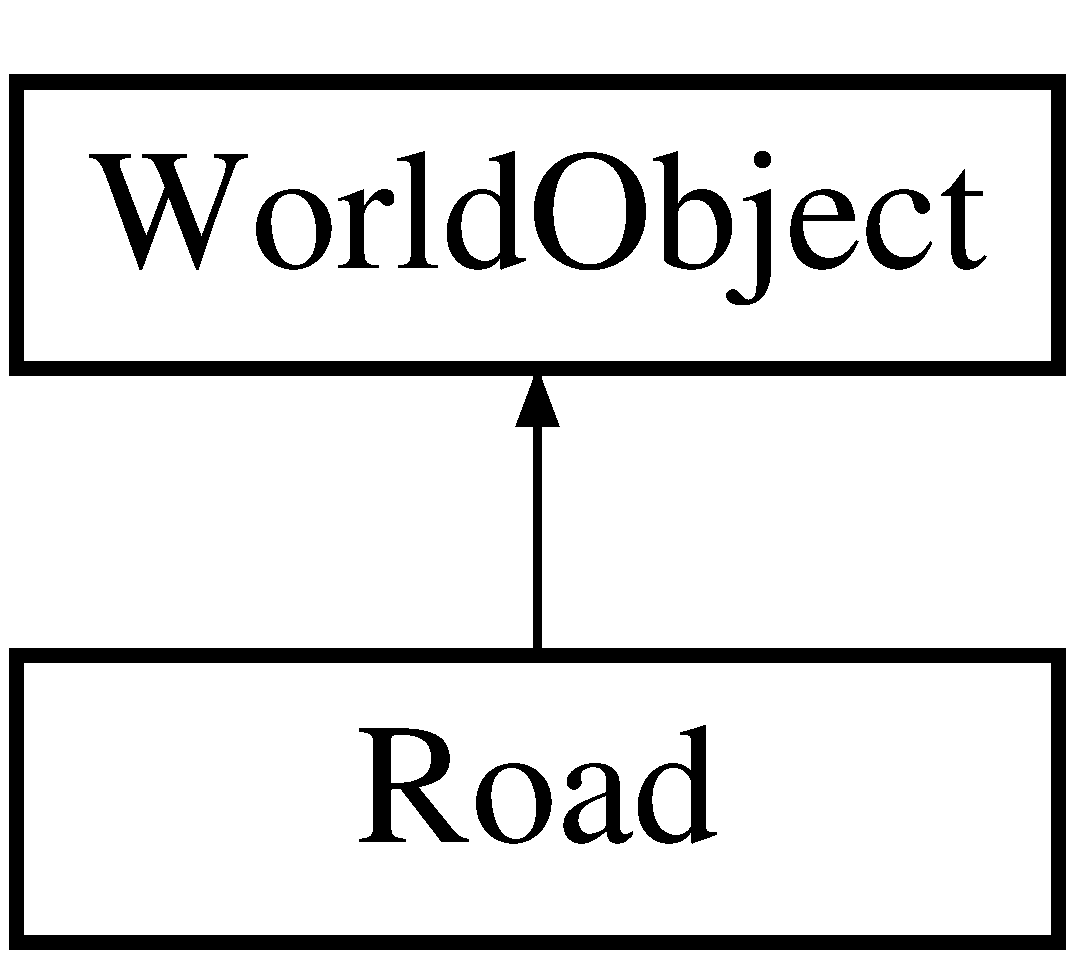
\includegraphics[height=2.000000cm]{class_road}
\end{center}
\end{figure}
\subsection*{Public Member Functions}
\begin{DoxyCompactItemize}
\item 
\hypertarget{class_road_a90be7d4371f8026017d3f6b819eeb688}{{\bfseries Road} (\hyperlink{struct_point3_d}{Point3\+D} x)}\label{class_road_a90be7d4371f8026017d3f6b819eeb688}

\item 
\hypertarget{class_road_adff20b6c1061106d116f624103650ec6}{void {\bfseries Draw\+Object} ()}\label{class_road_adff20b6c1061106d116f624103650ec6}

\item 
\hypertarget{class_road_a6e70d66fa043f061218a013a2a7c24c5}{\hyperlink{struct_point3_d}{Point3\+D} {\bfseries Get\+End\+Point} ()}\label{class_road_a6e70d66fa043f061218a013a2a7c24c5}

\end{DoxyCompactItemize}
\subsection*{Additional Inherited Members}


The documentation for this class was generated from the following files\+:\begin{DoxyCompactItemize}
\item 
Road.\+h\item 
Road.\+cpp\end{DoxyCompactItemize}

\hypertarget{class_scene}{\section{Scene Class Reference}
\label{class_scene}\index{Scene@{Scene}}
}
\subsection*{Public Member Functions}
\begin{DoxyCompactItemize}
\item 
\hypertarget{class_scene_a91913b921d41d374e00eac347358dc14}{void {\bfseries Render} ()}\label{class_scene_a91913b921d41d374e00eac347358dc14}

\item 
\hypertarget{class_scene_ac6ad6931a0fcbba7bdb60c105dbb9af2}{void {\bfseries Set\+Main\+Camera} (\hyperlink{class_camera}{Camera} $\ast$camera)}\label{class_scene_ac6ad6931a0fcbba7bdb60c105dbb9af2}

\item 
\hypertarget{class_scene_ac395fac38291f84eaf6cffd8458e6d95}{void {\bfseries Add\+Object} (\hyperlink{class_world_object}{World\+Object} $\ast$object)}\label{class_scene_ac395fac38291f84eaf6cffd8458e6d95}

\item 
\hypertarget{class_scene_ac0f05dc45b2bcec9f41f45ce79305116}{void {\bfseries Remove\+Object} (\hyperlink{class_world_object}{World\+Object} $\ast$object)}\label{class_scene_ac0f05dc45b2bcec9f41f45ce79305116}

\end{DoxyCompactItemize}


The documentation for this class was generated from the following files\+:\begin{DoxyCompactItemize}
\item 
Scene.\+h\item 
Scene.\+cpp\end{DoxyCompactItemize}

\hypertarget{class_sky}{\section{Sky Class Reference}
\label{class_sky}\index{Sky@{Sky}}
}
Inheritance diagram for Sky\+:\begin{figure}[H]
\begin{center}
\leavevmode
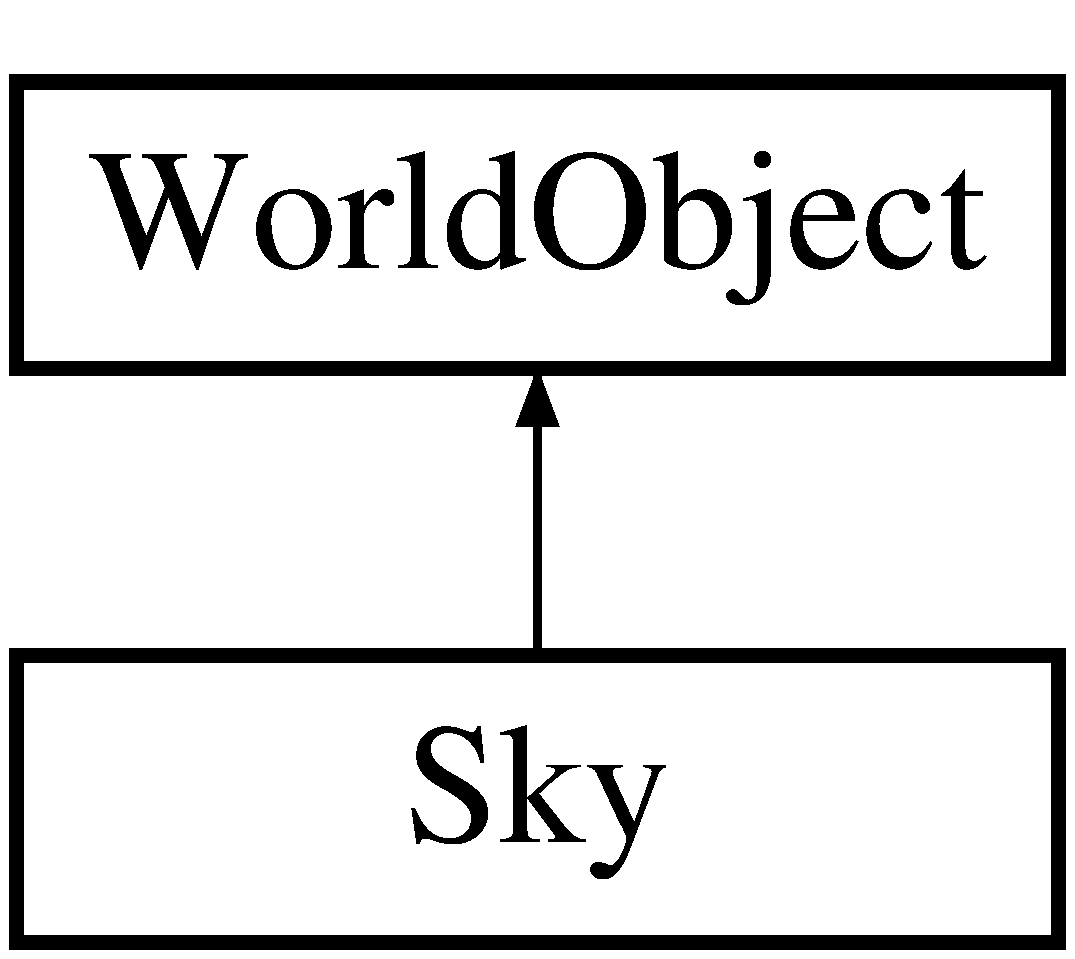
\includegraphics[height=2.000000cm]{class_sky}
\end{center}
\end{figure}
\subsection*{Public Member Functions}
\begin{DoxyCompactItemize}
\item 
\hypertarget{class_sky_a7969328d2fcbebdd7c7d456dc2a6cccd}{{\bfseries Sky} (G\+Lfloat size)}\label{class_sky_a7969328d2fcbebdd7c7d456dc2a6cccd}

\item 
\hypertarget{class_sky_afd761d9057943cc404448b3889e7e4f7}{void {\bfseries Follow} (\hyperlink{class_ball}{Ball} $\ast$ball)}\label{class_sky_afd761d9057943cc404448b3889e7e4f7}

\item 
\hypertarget{class_sky_ab2e87407bf02877b5375374990320cfc}{void {\bfseries Un\+Follow} ()}\label{class_sky_ab2e87407bf02877b5375374990320cfc}

\item 
\hypertarget{class_sky_a93a15559c1de7e0862d248933002620b}{void {\bfseries Update} ()}\label{class_sky_a93a15559c1de7e0862d248933002620b}

\end{DoxyCompactItemize}
\subsection*{Additional Inherited Members}


The documentation for this class was generated from the following files\+:\begin{DoxyCompactItemize}
\item 
Sky.\+h\item 
Sky.\+cpp\end{DoxyCompactItemize}

\hypertarget{class_textures}{\section{Textures Class Reference}
\label{class_textures}\index{Textures@{Textures}}
}
\subsection*{Public Member Functions}
\begin{DoxyCompactItemize}
\item 
\hypertarget{class_textures_a2eccc3b8d43e96e65af1b063fe642dc0}{G\+Luint $\ast$ {\bfseries Get\+Textures} ()}\label{class_textures_a2eccc3b8d43e96e65af1b063fe642dc0}

\item 
\hypertarget{class_textures_a130496e6fdd0da614bd4733cc18bb19f}{void {\bfseries Load\+G\+L\+Textures} ()}\label{class_textures_a130496e6fdd0da614bd4733cc18bb19f}

\end{DoxyCompactItemize}
\subsection*{Static Public Member Functions}
\begin{DoxyCompactItemize}
\item 
\hypertarget{class_textures_a3e5839f0cee717b4c7808a49ad9cf040}{static \hyperlink{class_textures}{Textures} $\ast$ {\bfseries Get\+Instance} ()}\label{class_textures_a3e5839f0cee717b4c7808a49ad9cf040}

\end{DoxyCompactItemize}


The documentation for this class was generated from the following files\+:\begin{DoxyCompactItemize}
\item 
Textures.\+h\item 
Main.\+cpp\item 
Textures.\+cpp\end{DoxyCompactItemize}

\hypertarget{class_tree}{\section{Tree Class Reference}
\label{class_tree}\index{Tree@{Tree}}
}


Derived from \hyperlink{class_plant}{Plant} class, indicates the pattern for creating each set of top points and the difference between each top's and base's radius.  




{\ttfamily \#include $<$Tree.\+h$>$}

Inheritance diagram for Tree\+:\begin{figure}[H]
\begin{center}
\leavevmode
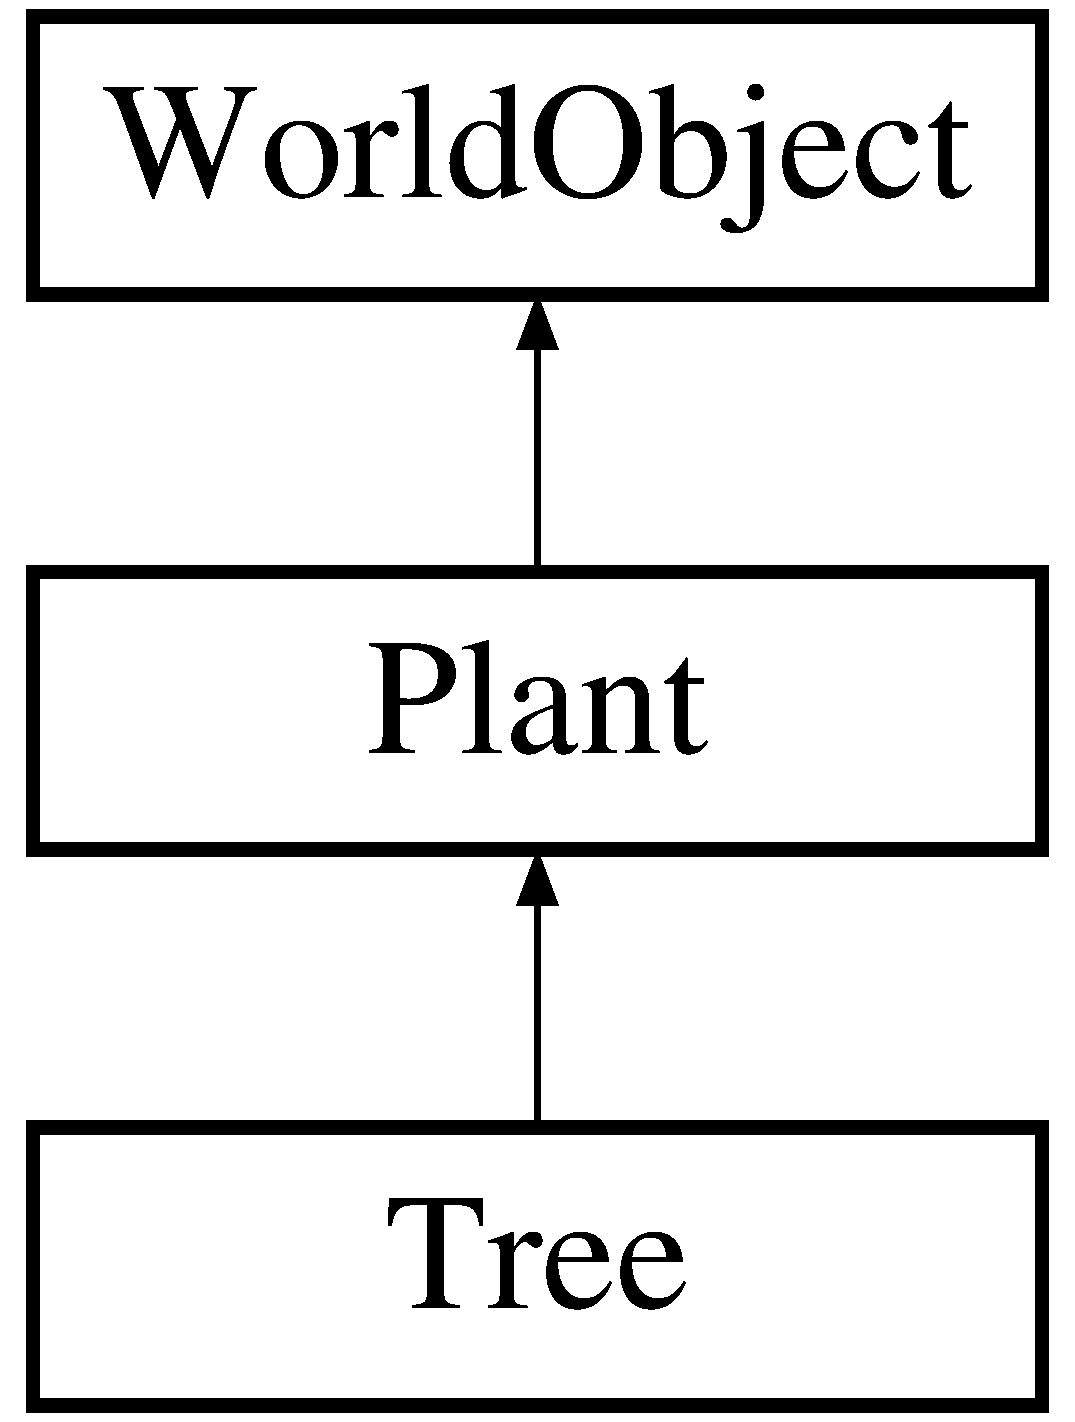
\includegraphics[height=3.000000cm]{class_tree}
\end{center}
\end{figure}
\subsection*{Public Member Functions}
\begin{DoxyCompactItemize}
\item 
\hyperlink{class_tree_a5f8726222034fdd427bf41abb2f1dced}{Tree} (double width, double height, int \hyperlink{class_plant_a4f86c46865d6211636140cef8805c6ee}{number\+Of\+Branches}, int \hyperlink{class_plant_ab49e92a2ab4ecdc762b5a1711fa3d65f}{level})
\item 
void \hyperlink{class_tree_ab0297a975c2e94b18773edb3e6eaf289}{Set\+Branch\+Top} (vector$<$ \hyperlink{struct_point3_d}{Point3\+D} $>$ base, vector$<$ \hyperlink{struct_point3_d}{Point3\+D} $>$ \&top, int current\+Level, G\+Lfloat \hyperlink{class_plant_abef0f751fe6b1b43ed208966a70b4ab3}{radius}, G\+Lfloat pass, G\+Lfloat index)
\item 
void \hyperlink{class_tree_afe594a748c525993d67ad51e005fc402}{Set\+Initial\+Pass} (G\+Lfloat \&pass, G\+Lfloat \hyperlink{class_plant_abef0f751fe6b1b43ed208966a70b4ab3}{radius})
\item 
void \hyperlink{class_tree_ae5a8dc3f5f4f94cd7cdf75ca1124cbc5}{Increment\+Pass} (G\+Lfloat \&pass, G\+Lfloat \hyperlink{class_plant_abef0f751fe6b1b43ed208966a70b4ab3}{radius})
\end{DoxyCompactItemize}
\subsection*{Additional Inherited Members}


\subsection{Detailed Description}
Derived from \hyperlink{class_plant}{Plant} class, indicates the pattern for creating each set of top points and the difference between each top's and base's radius. 

\subsection{Constructor \& Destructor Documentation}
\hypertarget{class_tree_a5f8726222034fdd427bf41abb2f1dced}{\index{Tree@{Tree}!Tree@{Tree}}
\index{Tree@{Tree}!Tree@{Tree}}
\subsubsection[{Tree}]{\setlength{\rightskip}{0pt plus 5cm}Tree\+::\+Tree (
\begin{DoxyParamCaption}
\item[{double}]{width, }
\item[{double}]{height, }
\item[{int}]{number\+Of\+Branches, }
\item[{int}]{level}
\end{DoxyParamCaption}
)}}\label{class_tree_a5f8726222034fdd427bf41abb2f1dced}
\hyperlink{class_tree}{Tree}'s constructor 
\begin{DoxyParams}{Parameters}
{\em width} & double -- The width of the surface \\
\hline
{\em height} & double -- The height of the surface \\
\hline
{\em number\+Of\+Branches} & int -- The number of branches \\
\hline
{\em level} & int -- The levels of branches \\
\hline
\end{DoxyParams}
Initializes the texture index. Generates a random value for the maximum height. Generates random values for directions, each branch's radius and angles for the rotations around Y and Z axis. Calculate the maximum height for the current branch. Generates the maximum heights for each branch.

\subsection{Member Function Documentation}
\hypertarget{class_tree_ae5a8dc3f5f4f94cd7cdf75ca1124cbc5}{\index{Tree@{Tree}!Increment\+Pass@{Increment\+Pass}}
\index{Increment\+Pass@{Increment\+Pass}!Tree@{Tree}}
\subsubsection[{Increment\+Pass}]{\setlength{\rightskip}{0pt plus 5cm}void Tree\+::\+Increment\+Pass (
\begin{DoxyParamCaption}
\item[{G\+Lfloat \&}]{pass, }
\item[{G\+Lfloat}]{radius}
\end{DoxyParamCaption}
)\hspace{0.3cm}{\ttfamily [virtual]}}}\label{class_tree_ae5a8dc3f5f4f94cd7cdf75ca1124cbc5}
Sets the value for incrementing the pass. 

Implements \hyperlink{class_plant}{Plant}.

\hypertarget{class_tree_ab0297a975c2e94b18773edb3e6eaf289}{\index{Tree@{Tree}!Set\+Branch\+Top@{Set\+Branch\+Top}}
\index{Set\+Branch\+Top@{Set\+Branch\+Top}!Tree@{Tree}}
\subsubsection[{Set\+Branch\+Top}]{\setlength{\rightskip}{0pt plus 5cm}void Tree\+::\+Set\+Branch\+Top (
\begin{DoxyParamCaption}
\item[{vector$<$ {\bf Point3\+D} $>$}]{base, }
\item[{vector$<$ {\bf Point3\+D} $>$ \&}]{top, }
\item[{int}]{current\+Level, }
\item[{G\+Lfloat}]{radius, }
\item[{G\+Lfloat}]{pass, }
\item[{G\+Lfloat}]{index}
\end{DoxyParamCaption}
)\hspace{0.3cm}{\ttfamily [virtual]}}}\label{class_tree_ab0297a975c2e94b18773edb3e6eaf289}
Initializes a vector of top points using a given base, its radius and a pass. 
\begin{DoxyParams}{Parameters}
{\em base} & vector$<$\+Point3\+D$>$ -- A vector that stores the points of the base of the branch \\
\hline
{\em top} & vector$<$\+Point3\+D$>$ -- A vector that will be initialized with the points of the top of the branch \\
\hline
{\em current\+Level} & int -- The current level of branches \\
\hline
{\em radius} & G\+Lfloat -- The radius of the base \\
\hline
{\em pass} & G\+Lfloat -- The difference between the radius of the base and the radius of the top \\
\hline
{\em index} & G\+Lfloat -- The index of the branch \\
\hline
\end{DoxyParams}
Calculates the difference between each top and base.

Initializes the top points on the left/right side according to the corresponding direction(1-\/left, 2-\/right). The radius of the top will be smaller than the radius of the base.

Implements \hyperlink{class_plant}{Plant}.

\hypertarget{class_tree_afe594a748c525993d67ad51e005fc402}{\index{Tree@{Tree}!Set\+Initial\+Pass@{Set\+Initial\+Pass}}
\index{Set\+Initial\+Pass@{Set\+Initial\+Pass}!Tree@{Tree}}
\subsubsection[{Set\+Initial\+Pass}]{\setlength{\rightskip}{0pt plus 5cm}void Tree\+::\+Set\+Initial\+Pass (
\begin{DoxyParamCaption}
\item[{G\+Lfloat \&}]{pass, }
\item[{G\+Lfloat}]{radius}
\end{DoxyParamCaption}
)\hspace{0.3cm}{\ttfamily [virtual]}}}\label{class_tree_afe594a748c525993d67ad51e005fc402}
Initializes the difference between top's and base's radius. 
\begin{DoxyParams}{Parameters}
{\em radius} & G\+Lfloat -- The radius of the base \\
\hline
{\em pass} & G\+Lfloat -- The difference between the radius of the base and the radius of the top \\
\hline
\end{DoxyParams}


Implements \hyperlink{class_plant}{Plant}.



The documentation for this class was generated from the following files\+:\begin{DoxyCompactItemize}
\item 
Tree.\+h\item 
Tree.\+cpp\end{DoxyCompactItemize}

\hypertarget{class_world_object}{\section{World\+Object Class Reference}
\label{class_world_object}\index{World\+Object@{World\+Object}}
}
Inheritance diagram for World\+Object\+:\begin{figure}[H]
\begin{center}
\leavevmode
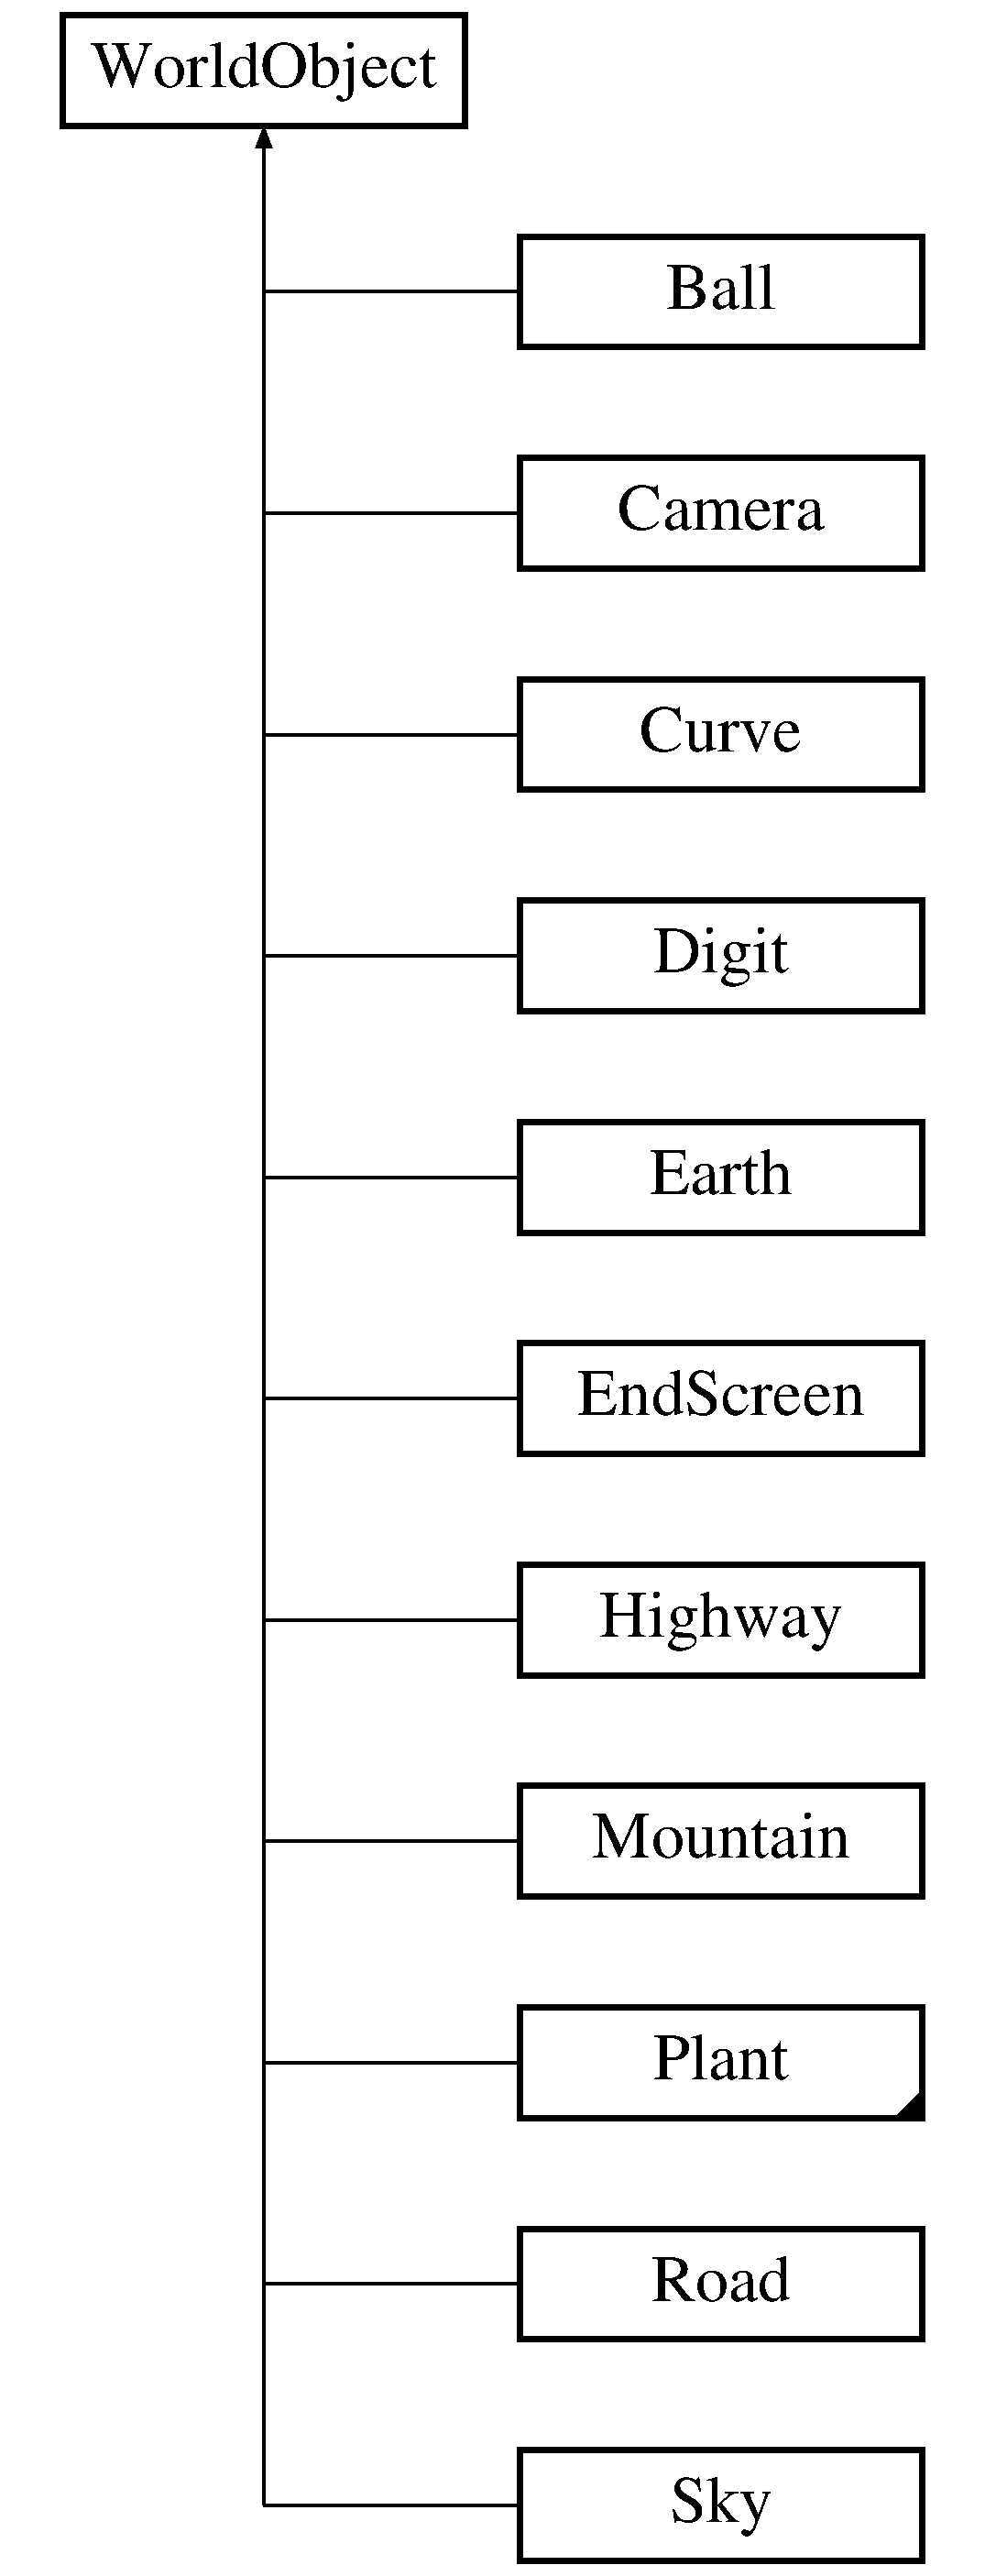
\includegraphics[height=12.000000cm]{class_world_object}
\end{center}
\end{figure}
\subsection*{Public Member Functions}
\begin{DoxyCompactItemize}
\item 
\hypertarget{class_world_object_a464fd2e8938ae8ca4e778235819d616a}{{\bfseries World\+Object} (G\+Lfloat W=0.\+0, G\+Lfloat H=0.\+0, G\+Lfloat X=0.\+0, G\+Lfloat Y=0.\+0, G\+Lfloat Z=0.\+0)}\label{class_world_object_a464fd2e8938ae8ca4e778235819d616a}

\item 
\hypertarget{class_world_object_ab70b8fbf6ec1c1d9fe6a95c791c321f3}{void {\bfseries Translate} (\hyperlink{struct_point3_d}{Point3\+D})}\label{class_world_object_ab70b8fbf6ec1c1d9fe6a95c791c321f3}

\item 
\hypertarget{class_world_object_adc741ef57132da4aa8cbac78db3fff26}{void {\bfseries Rotate} (\hyperlink{struct_point3_d}{Point3\+D})}\label{class_world_object_adc741ef57132da4aa8cbac78db3fff26}

\item 
\hypertarget{class_world_object_ae46caed8b37233c2b9e0383a26cb9f87}{void {\bfseries Draw} ()}\label{class_world_object_ae46caed8b37233c2b9e0383a26cb9f87}

\item 
\hypertarget{class_world_object_a3a3158dc13f636eb3835e22fdc32a7b9}{\hyperlink{struct_point3_d}{Point3\+D} {\bfseries Get\+Forward} ()}\label{class_world_object_a3a3158dc13f636eb3835e22fdc32a7b9}

\item 
\hypertarget{class_world_object_aff5a65911deeaedf114357217d16c66f}{\hyperlink{struct_point3_d}{Point3\+D} {\bfseries Get\+Translate} ()}\label{class_world_object_aff5a65911deeaedf114357217d16c66f}

\item 
\hypertarget{class_world_object_aba6fb82b134193bdcb5882a7e83e937a}{\hyperlink{struct_point3_d}{Point3\+D} {\bfseries Get\+Right} ()}\label{class_world_object_aba6fb82b134193bdcb5882a7e83e937a}

\item 
\hypertarget{class_world_object_a443ed580b100165115e4fd2d7cdaae43}{\hyperlink{struct_point3_d}{Point3\+D} {\bfseries Get\+Rotate} ()}\label{class_world_object_a443ed580b100165115e4fd2d7cdaae43}

\end{DoxyCompactItemize}
\subsection*{Protected Member Functions}
\begin{DoxyCompactItemize}
\item 
\hypertarget{class_world_object_a22d6db7c7f7ac55f873d55417417d29d}{virtual void {\bfseries Draw\+Object} ()=0}\label{class_world_object_a22d6db7c7f7ac55f873d55417417d29d}

\item 
\hypertarget{class_world_object_a52db8a34a804e30a25043b8b118b3365}{void {\bfseries Modify\+Perspective} ()}\label{class_world_object_a52db8a34a804e30a25043b8b118b3365}

\item 
\hypertarget{class_world_object_a4873b7b568e1ce3886092823834c16b3}{void {\bfseries Modify\+Perspective\+Back} ()}\label{class_world_object_a4873b7b568e1ce3886092823834c16b3}

\end{DoxyCompactItemize}
\subsection*{Protected Attributes}
\begin{DoxyCompactItemize}
\item 
\hypertarget{class_world_object_ac6a87c572496ee57740aff2bf4cb7c07}{\hyperlink{struct_point3_d}{Point3\+D} {\bfseries rotate}}\label{class_world_object_ac6a87c572496ee57740aff2bf4cb7c07}

\item 
\hypertarget{class_world_object_a3e290757727e835e6a075d2565e093a7}{\hyperlink{struct_point3_d}{Point3\+D} {\bfseries translate}}\label{class_world_object_a3e290757727e835e6a075d2565e093a7}

\item 
\hypertarget{class_world_object_aa4d4ce305467868cdbb17fc25759408f}{G\+Lfloat {\bfseries width}}\label{class_world_object_aa4d4ce305467868cdbb17fc25759408f}

\item 
\hypertarget{class_world_object_a0457012633125921dd5c43e8538e8674}{G\+Lfloat {\bfseries height}}\label{class_world_object_a0457012633125921dd5c43e8538e8674}

\end{DoxyCompactItemize}


The documentation for this class was generated from the following files\+:\begin{DoxyCompactItemize}
\item 
World\+Object.\+h\item 
World\+Object.\+cpp\end{DoxyCompactItemize}

%--- End generated contents ---

% Index
\newpage
\phantomsection
\addcontentsline{toc}{chapter}{Index}
\printindex

\end{document}
